%%% Results %%%
\chapter{Results} \label{ch:results}
 We implement Monte-Carlo algorithm \ref{sec:myalgorithm} in C++ and push to the open GitHub repository \cite{gitsaw}. Numerical simulations were done using the computational resources of HPC facilities at HSE University \cite{Kostenetskiy_2021}.
 
 
 
\section{XY model on SAWs, 2D}
To perform MC simulations for short chains from $N=100$ to $N=1000$, we run at least $2.1 \times 10^9$ MC steps using two  types of updates: snake-like and reconnect. We choose following update probabilities: $P_{local}=0.8$, $P_{reconnect}=0.2$. 

For longer chains $N>1000$ we additionally use cluster update. We simulate chains up to $N=4900$. For $N=4900$, we run at least $8 \times 10^{10} $ MC steps. Here we use these values for update probabilities: $P_{local}=0.8$, $P_{reconnect}=0.199$, $P_{Wolff}=0.001$. Despite both Reconnect and Cluster  updates  have complexity $O(N)$, we choose small $P_{Wolff}$ due to slow iterations cause by using queue for creating cluster of spins. At average, the Reconnect is much faster and leads to get faster convergence of geometry properties, for example, mean radius. 

 
\subsection{Tests for validation simulations}
To test our Monte-Carlo (M) simulation, we compare results obtained using MC and Sampling + Exact Enumeration (EE). The exact numeration is the generation of all self-avoiding walks of the particular low value $N$ using recursion technique. As the space of spin configuration is continuous, we simply sample a number of vectors which components come from the uniform distribution $U(-\pi, \pi)$. For each generated SAW-conformation we generate the set of spin configurations. This allows to obtain mean values and sum generated sets to the partition function. This method is only approximation, but it helps to make approximate checks. 

We calculate Mean Radius \eqref{endtoend}, mean energy \eqref{hamiltonian} and   second moment of magnetization \eqref{secondmomentmagnetization} for short chains ($N=5, N=8$).  The generation of spin configuration and applied it to the whole set of SAWs is resource-consuming procedure. Therefore, we sample spin configurations only $600$ times (so, 600 sequences of spins applied to each conformation) and repeat this $10$ times. Figure \ref{fig:ee} shows obtained results.  For $J=0$, the second moment of magnetization are close to exact values \eqref{m2j0} and the mean energy starts at $\langle e \rangle = 0$. Therefore, teh MC data in a good accordance with the expected values from Section \ref{U4J0}. 

 \begin{figure} 
	\centering
	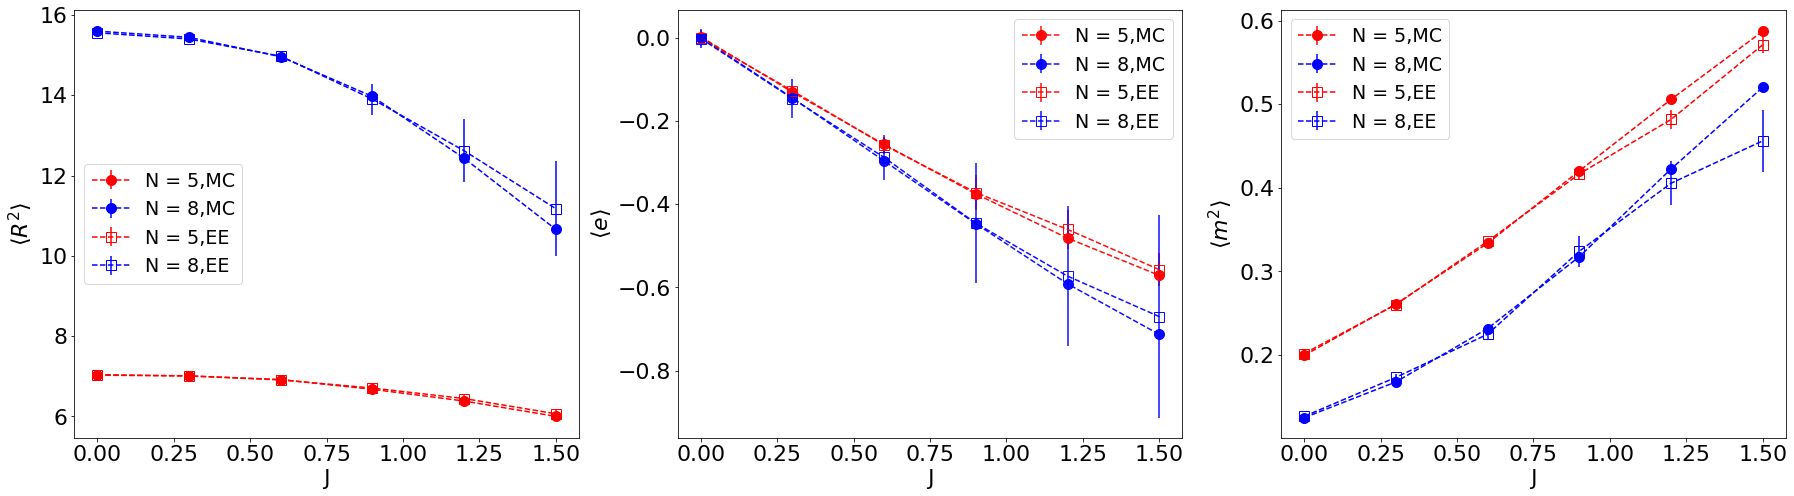
\includegraphics[scale=0.26]{Images/EE.png}
	\caption{  Mean Radius \eqref{endtoend}, mean energy \eqref{hamiltonian} and   second moment of magnetization \eqref{secondmomentmagnetization}.   }
	\label{fig:ee}
\end{figure}

The other way to validate implemented algorithm is to vary set of probabilities for updates which we denote as $(p_1,p_2,p_3)= (P_{local},P_{reconnect},P_{Wolff}$. The most important region for checking is critical region where physical quantities are dynamic. For non-interacting regime, the program could give correct values predicted analytically, but it does not help to avoid bugs in energy-dependent steps in iterations, such as calculating acceptance probability. For large $J$ in should-be-compact-maybe-ordered phase, the physical properties are also quite stable and bugs are less obvious.  It is a tricky moment that we need to have a correct implementation to find the critical region, but we need to know the critical interval to validate programmed code and be sure that it is correct implementation. However, we can overcome it over iterations and narrowing critical region running short simulations for short chains. 

To make final check of the written code for simulations, we run program for two chains lengths $N=500$ and $N=700$ at the narrowed region where the critical behavior is expected from previous short run. We vary $J$ and perform simulations using four sets of $(p_1,p_2,p_3)$. In two stets we do not use Cluster update to check its implementation separately. Figure \ref{fig:MCdiffP} illustrates results of validation for three properties, mean Radius \eqref{endtoend}, mean energy \eqref{hamiltonian}, second moment of magnetization \eqref{secondmomentmagnetization} as a functions of coupling constant $J$. For both lengths, the curves for each function overlap within combined errorbars. 


 \begin{figure} 
	\centering
	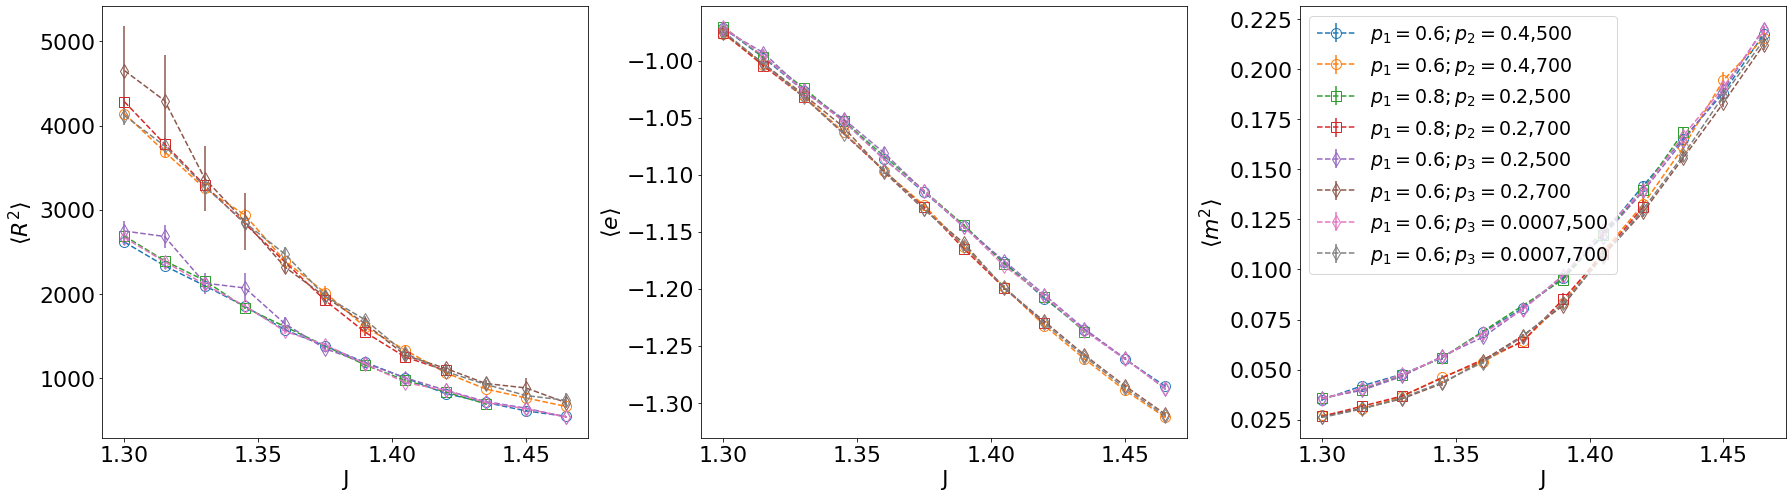
\includegraphics[scale=0.26]{Images/tests_2D.png}
	\caption{ Mean Radius \eqref{endtoend}, mean energy \eqref{hamiltonian} and   second moment of magnetization \eqref{secondmomentmagnetization} as functions of $J$ on the critical region for two chains lengths $N=500$ and $N=700$. $(p_1 + p_2 + p_3 = 1 $  }
	\label{fig:MCdiffP}
\end{figure}


\subsection{Thermodynamic properties}
First, we measure the mean square magnetization \eqref{secondmomentmagnetization} and the mean energy \eqref{hamiltonian} for short chains (up to $N=1000$) in the large range of the interaction energy $J$ and for long chains (up to $N=4900$) in the narrow range where the system are expected to undergo the phase transition.

 \begin{figure}[!ht]
	\centering
	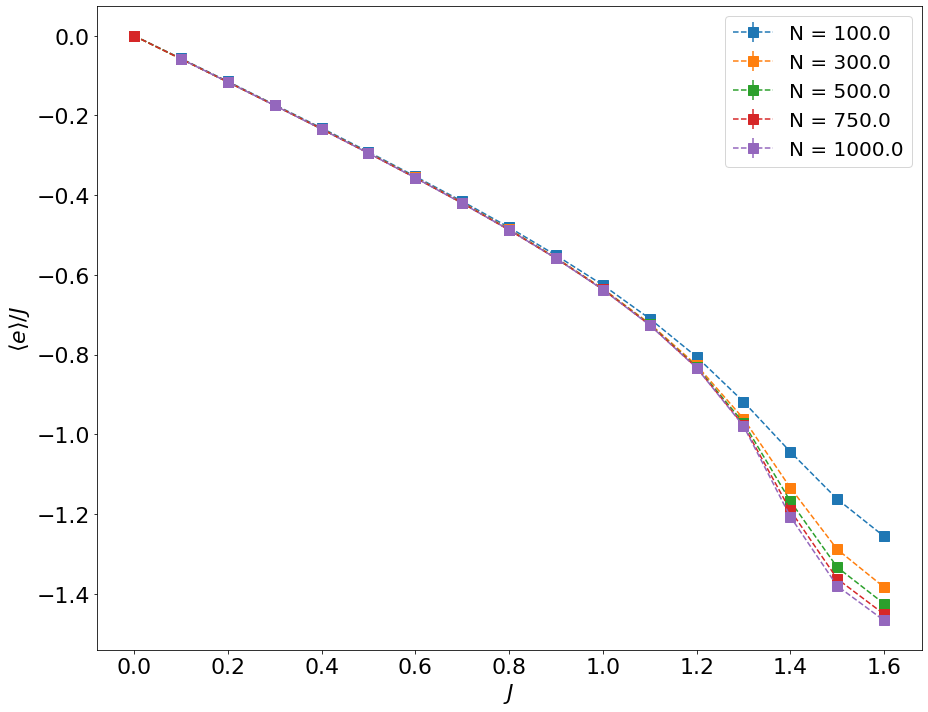
\includegraphics[scale=0.23]{Images/energy_shortchains.png}
	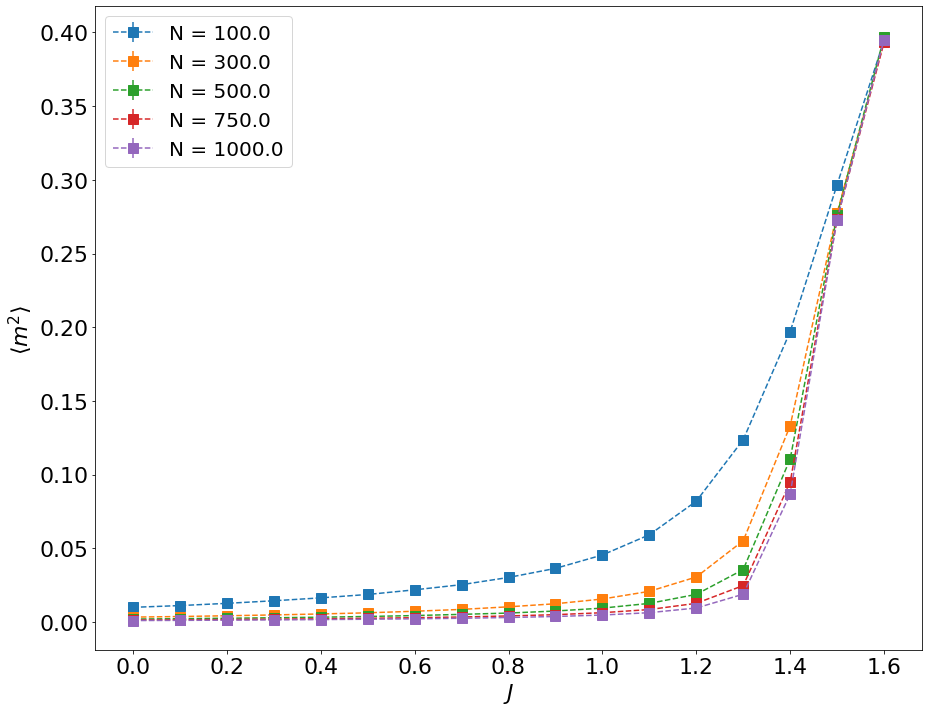
\includegraphics[scale=0.23]{Images/magnetization2_shortchains.png} \\
	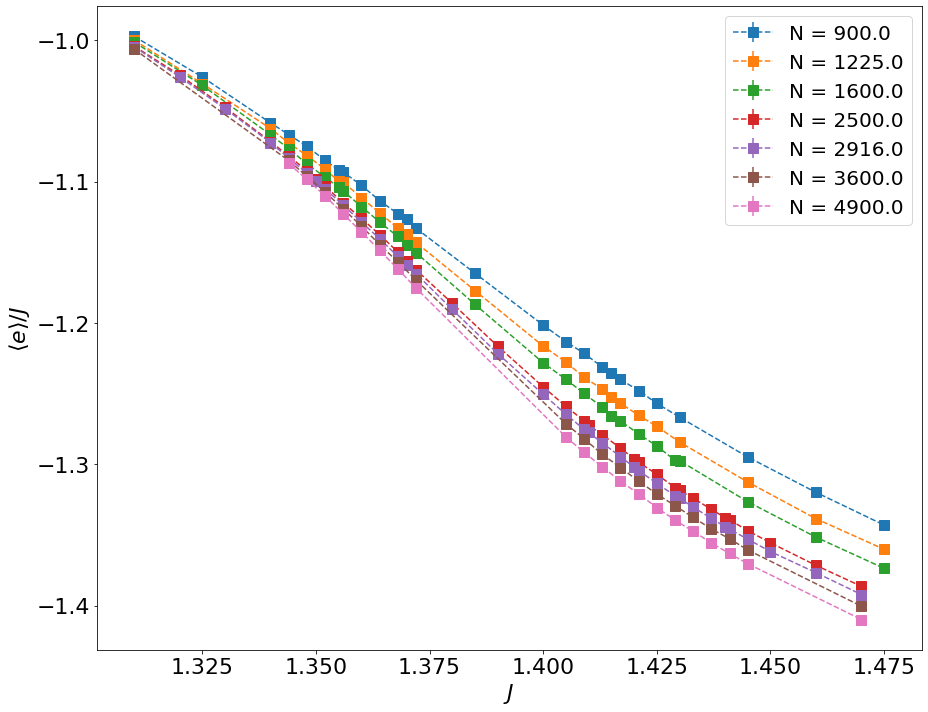
\includegraphics[scale=0.23]{Images/energy_longchains.png}
	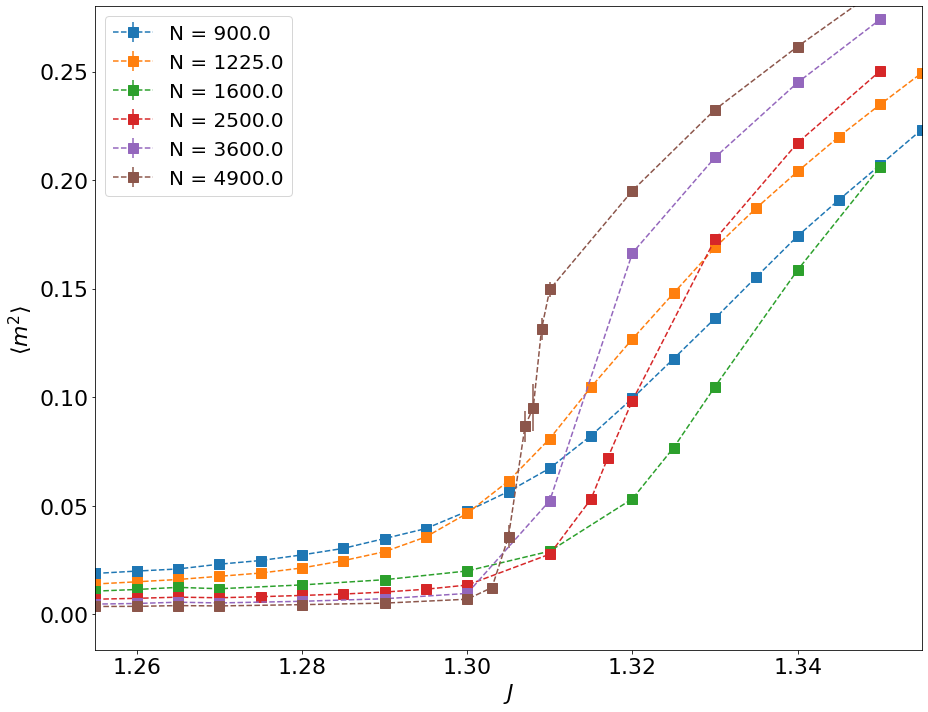
\includegraphics[scale=0.23]{Images/magnetization2_longchains.png}
	\caption{$h=0$. Mean energy \eqref{hamiltonian} and   second moment of magnetization \eqref{secondmomentmagnetization}. Symbols are MC data with errors with dashed line as a guide to the eye. }
	\label{fig:energymagshort}
\end{figure}

 Figure \ref{fig:energymagshort} (left column) shows computational results for the mean energy  \eqref{hamiltonian} as a function of $J$. At the top plot for short chains, the mean energy starts at $\langle e \rangle = 0$ as expected for unfolded disordered SAWs. %As $N \rightarrow \infty$, the value of the mean energy decreases and goes to the asymptotic value $\langle e \rangle = -2J$ for compact ordered walk. 
 
  Figure \ref{fig:energymagshort} (right column) illustrates obtained numerical results for the second moment of magnetization \eqref{secondmomentmagnetization}. At $J=0$, results are consisted with the exact solution \eqref{m2j0} and $  \langle m^2 \rangle  \rightarrow 0$ as $N \rightarrow \infty$. As $J$ increases, the square of magnetization grows up. One can expect an ordering behavior for large J.
  
  %From both energy and the second magnetization moment, we can clearly see the finite size effect. The longer chains has jumps in the function for lower $J$ in comparison to shorter ones. 
 
 
%Figure \ref{fig:energymagshort} illustrates obtained results for Mean energy \eqref{hamiltonian} and   second moment of magnetization \eqref{secondmomentmagnetization}. The system tends to order as interaction energy $J$ gets larger. 
\subsection{Structural properties}

 \begin{figure}[!ht]
	\centering
	\captionsetup{justification=centering}
	\begin{subfigure}[b]{0.45\textwidth}
		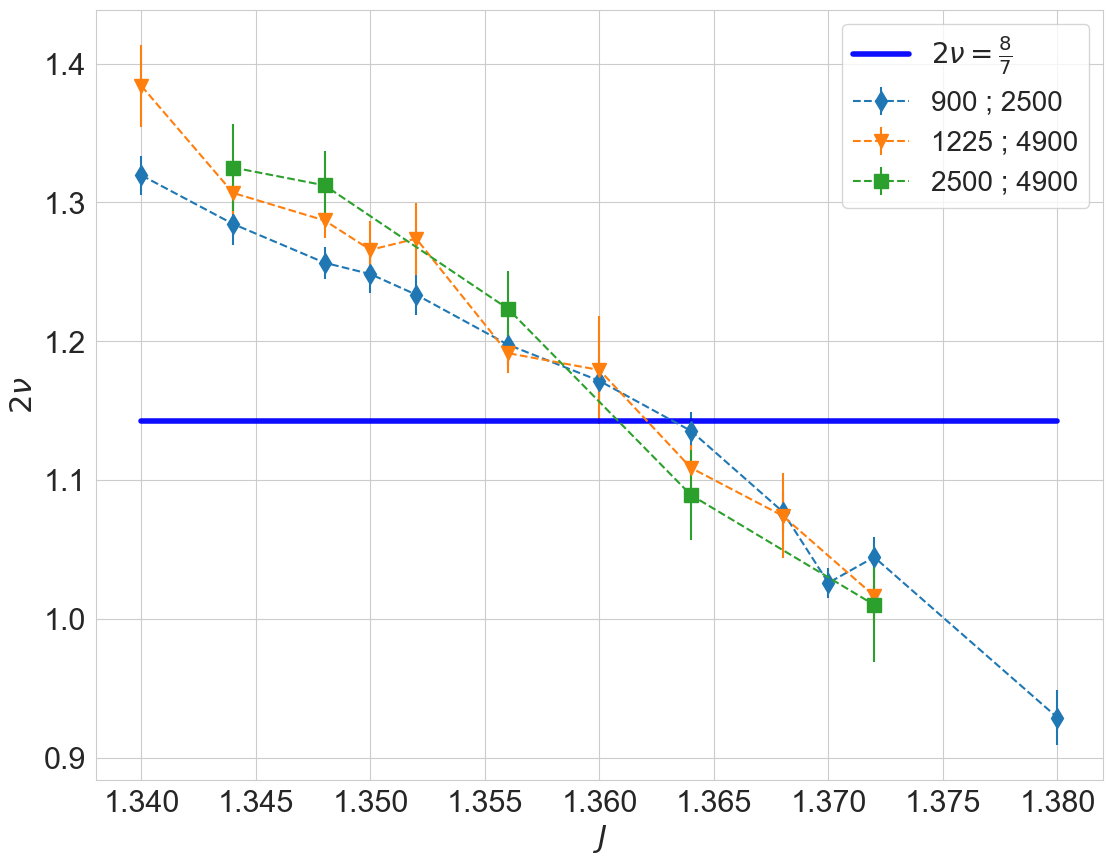
\includegraphics[width=\textwidth]{Images/nucross_longchains.png}
		\caption{ Scaling function \eqref{varphir} as a function of $J$. The errorbars are computed via Gaussian sampling. }
		\label{fig:Rscaled_wide}
	\end{subfigure}
	\begin{subfigure}[b]{0.45\textwidth}
		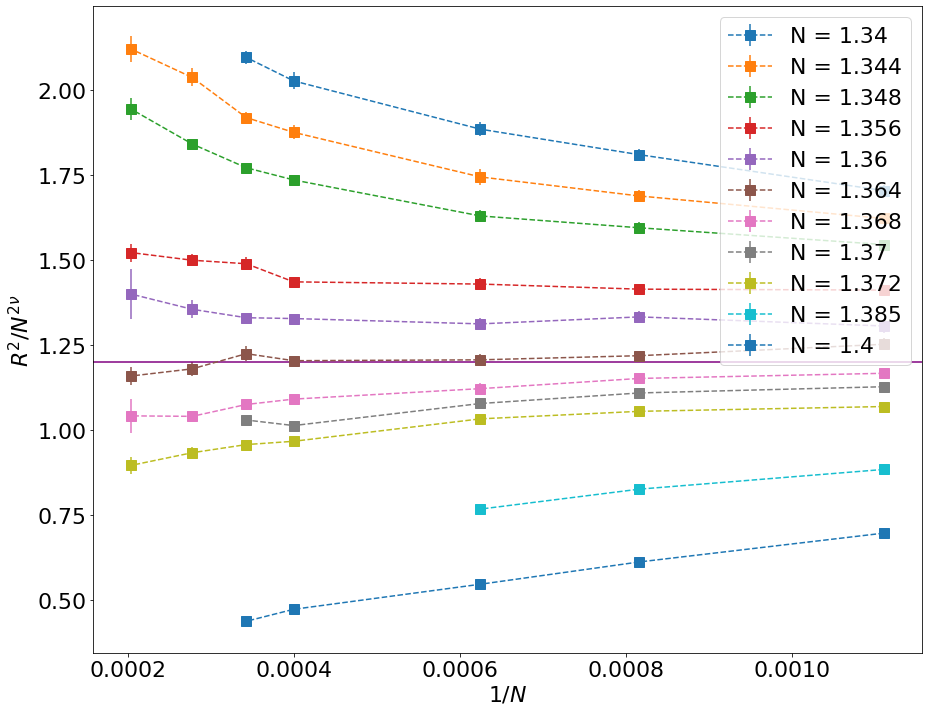
\includegraphics[width=\textwidth]{Images/rscaling_longchainscross.png}
		\caption{Scaled Mean-squared end-to-end distance using $\nu_{\theta}=4/7$ as a function of $1/N$ from $N=900$ to $N=4900$.}
		\label{fig:Rscaled_narrow}
	\end{subfigure}
	\caption{ Visual inspection of scaling of mean radius.  The  purple horizontal line corresponds to structural phase transition.  
	}
	\label{fig:Rscaled}
\end{figure}


We start our studying structural properties of the model with visual inspection of the scaling function for mean radius \eqref{varphir}. We calculate scaling ratios for different pairs of chain lengths $N_1,N_2$. In the model of classical interacting SAWs without spins, the curves cross at the structural phase transition point and at the critical value of exponent $\nu$. In this step, our obtained computational data for XY on SAWs \ref{fig:Rscaled_wide} do not contradict the assumption that value $\nu$ is inherited from the iSAW model. However, we cannot make estimation of crossing point due to large errorbars. 

Figure \ref{fig:Rscaled_narrow} shows the scaled
mean-squared end-to-end distance by $\nu=4/7$ as a function of 
$1/N$ for different $J$. The horizontal line is placed at the estimation from Section \ref{sec:2DJthetatransition}. This line corresponds to the structural phase transition point.

\label{structureprocedure}
Next, we estimate critical exponent $\nu$ \eqref{r_scale} from the asymptotic power law for the mean square end-to-end distance of SAWs. We use following ansatz  \cite{Berretti1985}:
\begin{equation}
\label{berettiscale}
\log (R_N^2+k_1 ) = 2 \nu \log (N+k_2) + b.
\end{equation}
Here $k_1=k_2=1$ are phenomenological parameters. 
 \begin{figure} 
 	\centering
 	\captionsetup{justification=centering}
\begin{subfigure}[b]{0.45\textwidth}
	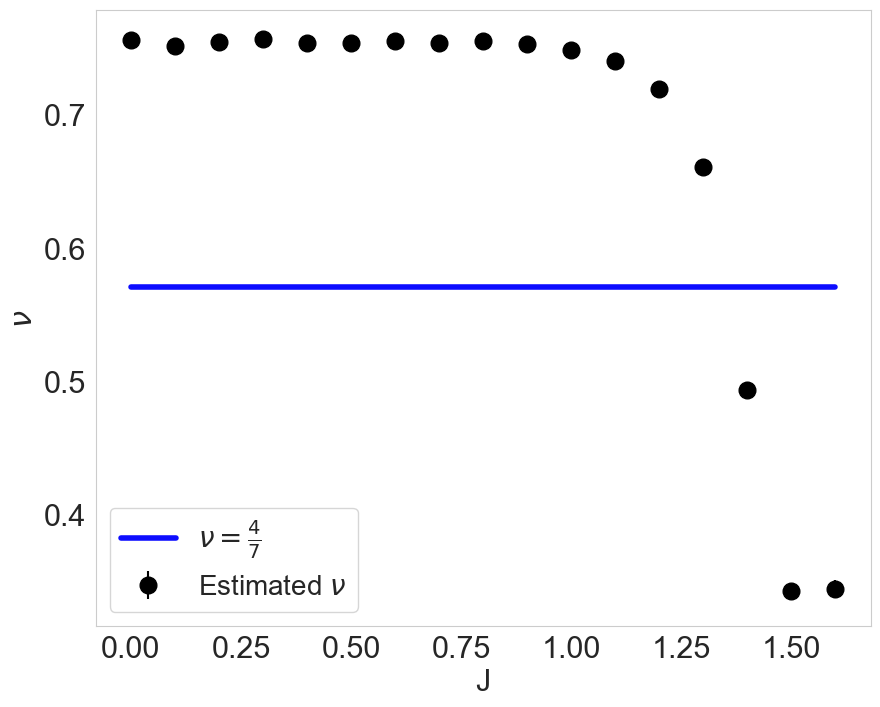
\includegraphics[scale=0.36]{Images/nu_shortchains.png}
	\centering{\caption{ From $N=100$ to $N=1000$. } }
	\label{fig:nushort_left}
\end{subfigure}
	\begin{subfigure}[b]{0.45\textwidth}
	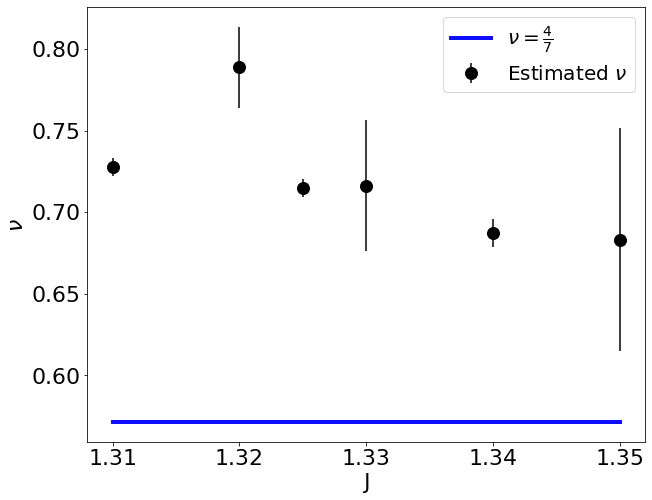
\includegraphics[scale=0.36]{Images/nu_shortchains_1.png}
		\caption{ From $N=1225$ to $N=4900$. }
	\label{fig:nushort_right}
\end{subfigure}
	\caption{  Estimates with errorbars of critical exponent $\nu$ via \eqref{berettiscale} .   }
	\label{fig:nushort}
\end{figure}
 

For the start, we perform curve-fitting for short chains on the large range of values $J$. Figure \ref{fig:nushort} illustrates obtained results of exponent estimation. In $J=0$, the critical exponent $\nu$ equals $\nu = \frac{3}{4}$  which is consisted with the value of non-interacting SAWs \eqref{nur}. The value $\nu=\frac{4}{7}$, which is the exact value
for interacting SAWs \eqref{nu_theta}, appears at the region $ 1.25 < J < 1.4$ (Figure \ref{fig:nushort}, left part). Despite effects of finite size, we can create the idea that structural phase transition happens at the $J \in [1.32; 1.37]$ (Figure \ref{fig:nushort}, right part).  %In previous section we showed that the energy and second magnetization moment functions of $J$ have jumps approximately at the same region. 

  We thus use that XY model on SAWs also has value $\nu = 4/7$ \eqref{nu_theta} at the point of structural phase transition. We use this value to obtain collapsing plots in Figure \ref{fig:bcshort} in following subsection \ref{section:Transition}. 

%\section{Scalings}
%Next, we move to estimation of the crossover exponent $\phi$ which
%quantifies the deviation from criticality via the scaled coupling $x = (J-J_c) / N^{-\phi}$ \cite{van2015statistical}. In \cite{PhysRevE.104.024122, PhysRevE.104.054501} it was assumed the value $\phi \approx 0.71$. We use this value to produce scaling plots \ref{fig:radiusscaling}. 
%\begin{figure}[H]
%	\centering
%	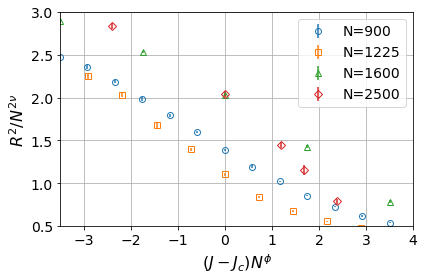
\includegraphics[scale=0.23]{Images/R2_data_collapse_phi.png} 	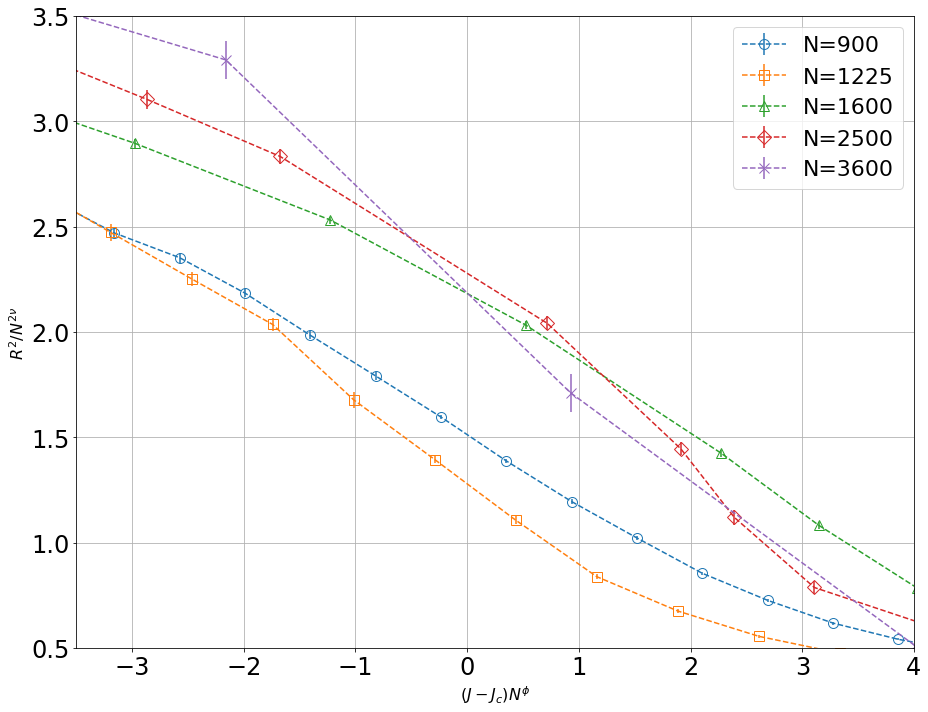
\includegraphics[scale=0.23]{Images/R2_data_collapse_phi1.png} \\ 
%	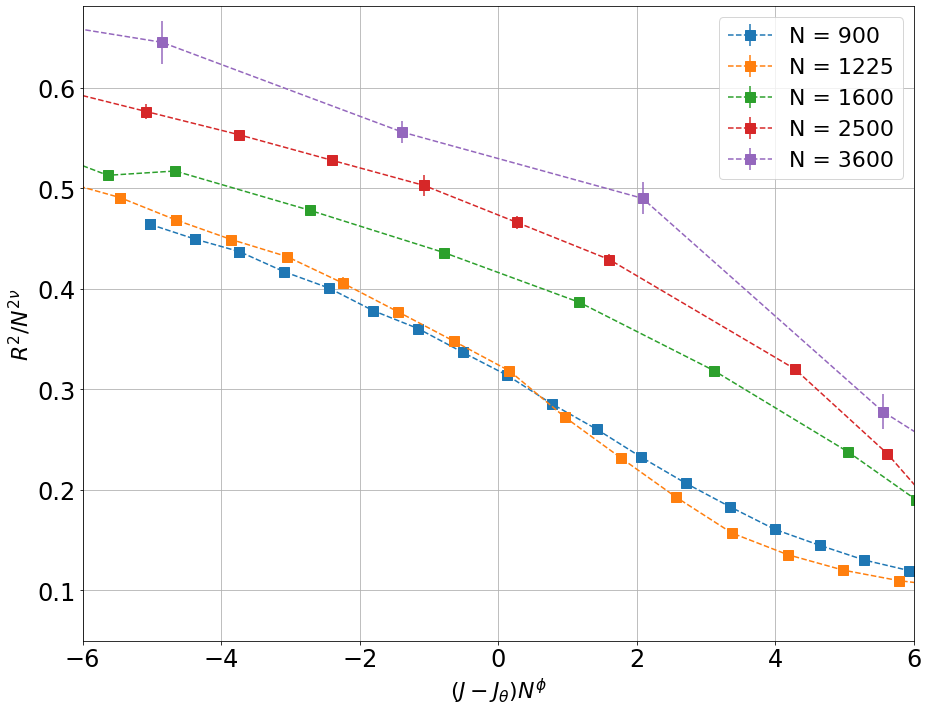
\includegraphics[scale=0.23]{Images/rscalinglong_dc.png}
%	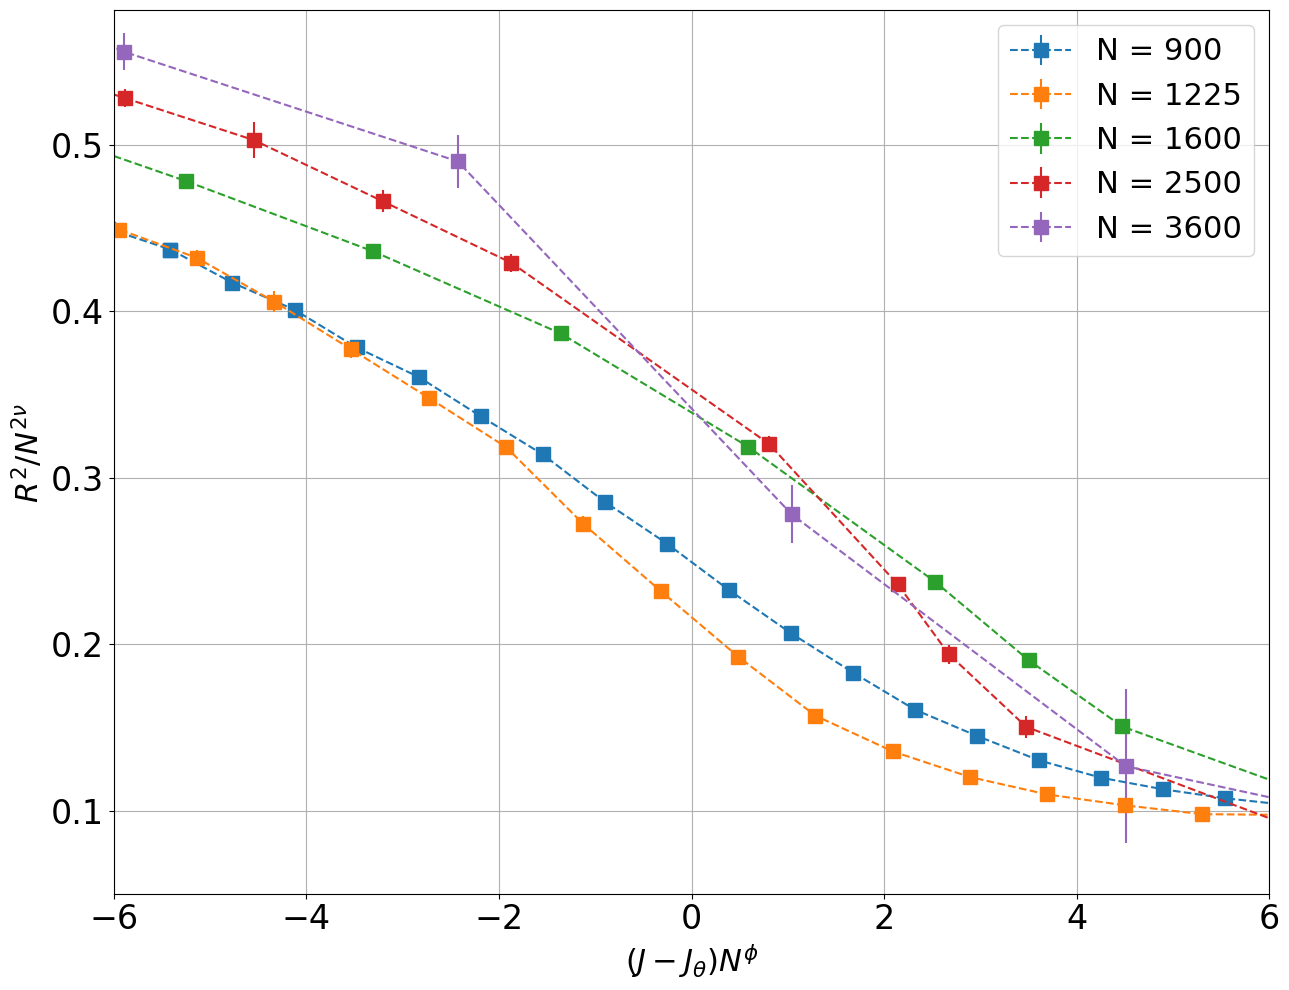
\includegraphics[scale=0.23]{Images/rscalinglong_dc1.png} 	\\
%		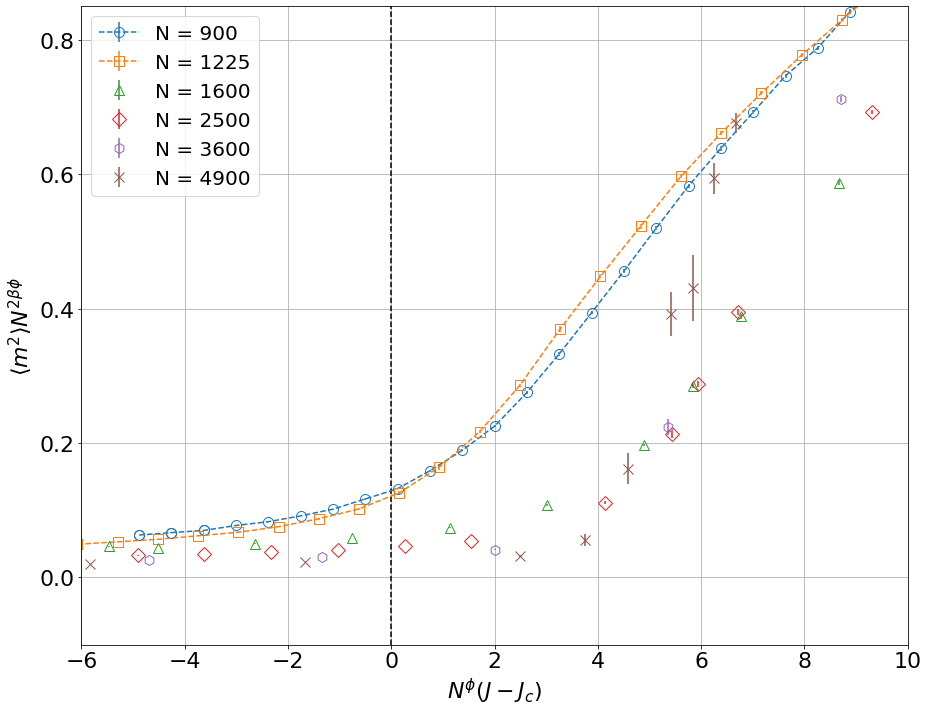
\includegraphics[scale=0.23]{Images/2dmag2scaling.png} 	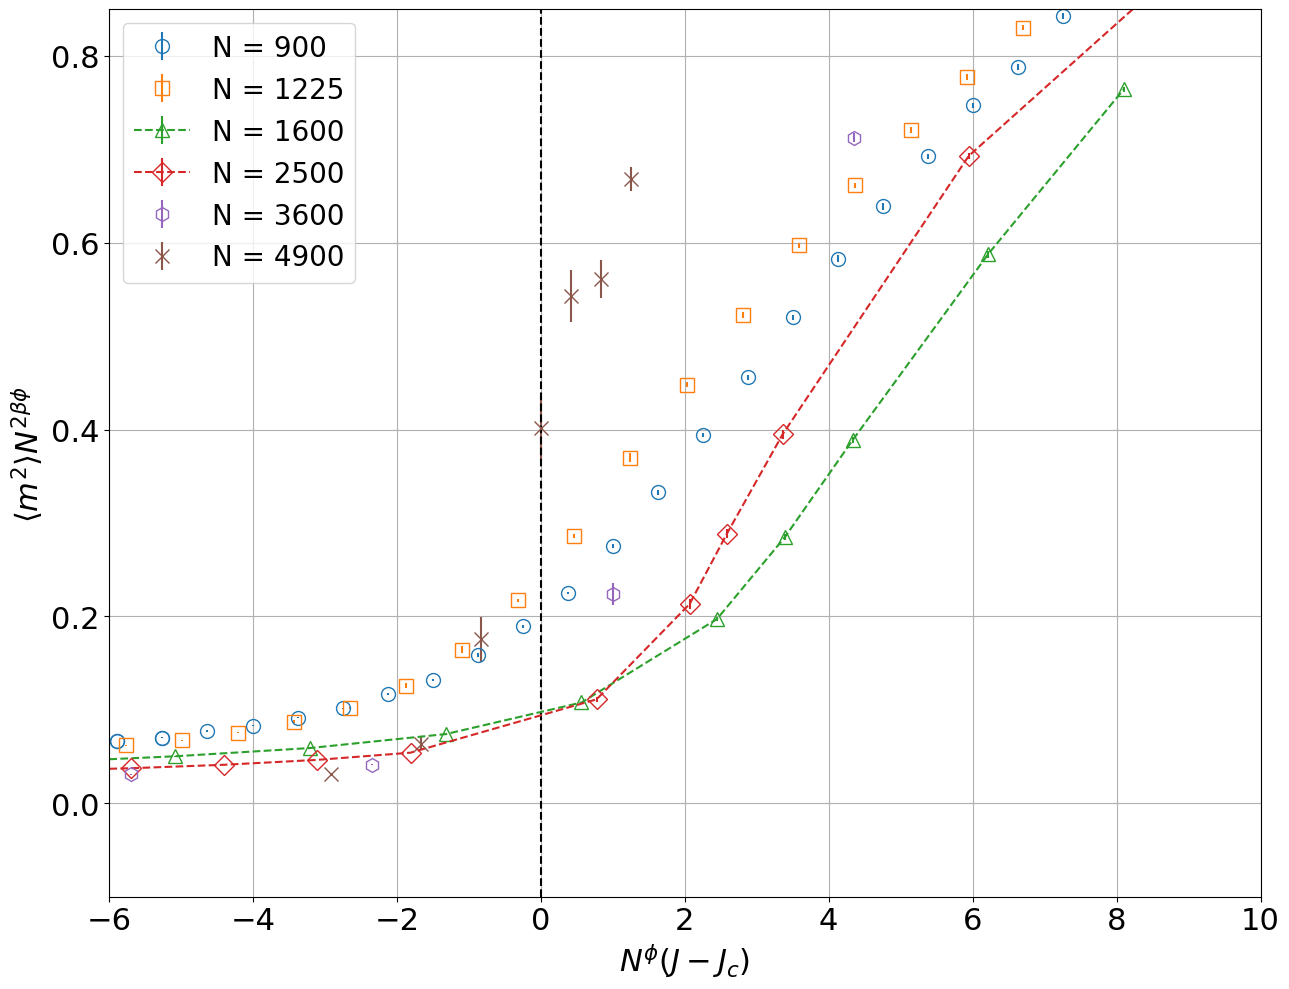
\includegraphics[scale=0.23]{Images/2dmag2scaling1.png}  
%	\caption{$h=0$. Mean radius \eqref{endtoend} and second moment of magnetization \eqref{secondmomentmagnetization} scalings. For left plots we use value $J_{\theta}=1.294$ and for right plots $J_{theta}=1.307$. We assume $\phi=5/7$. }
%	\label{fig:radiusscaling}
%\end{figure}
\subsection{Transition} \label{section:Transition}
To focus on studying phase transition, we calculate two characteristics. The first one is the mean square end-to-end distance scaled using the factor $\nu = \frac{4}{7}$ in \eqref{r_scale}. The second one is Binder cumulant of magnetization \eqref{binderqum}. Figure \ref{fig:bcshort}  presents obtained calculations. 

 \begin{figure}[!ht]
	\centering
	\captionsetup{justification=centering}
	\begin{subfigure}[b]{0.45\textwidth}
		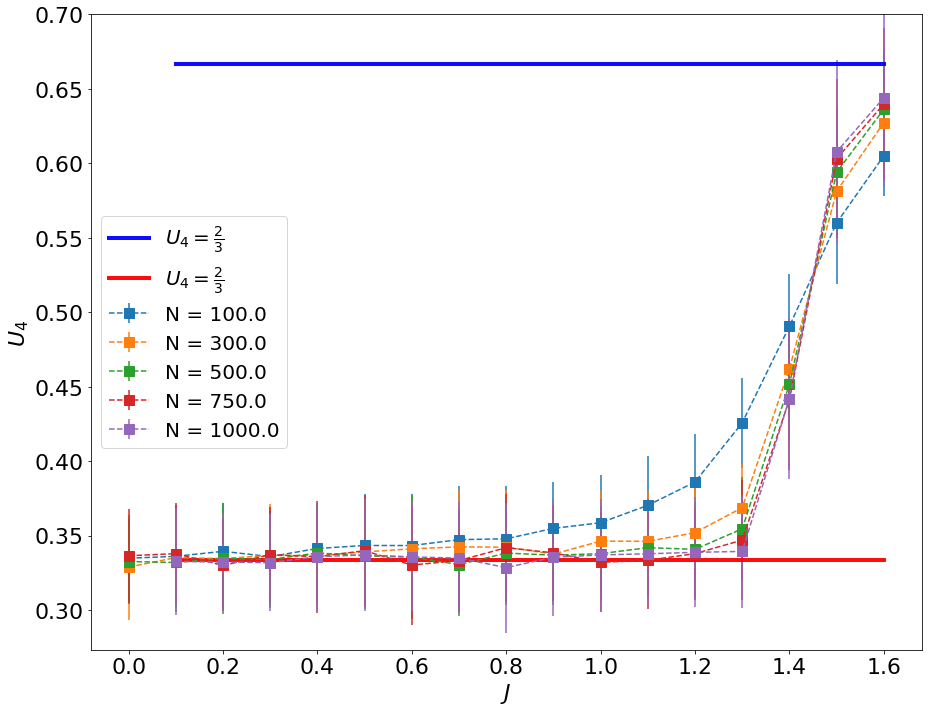
\includegraphics[width=\textwidth]{Images/bindercumulants_shortchains.png}
		\caption{ Binder cumulant on the wide range of J with both lower and upper limits.  }
		\label{fig:bcshort_shortbc}
	\end{subfigure}
	\begin{subfigure}[b]{0.45\textwidth}
		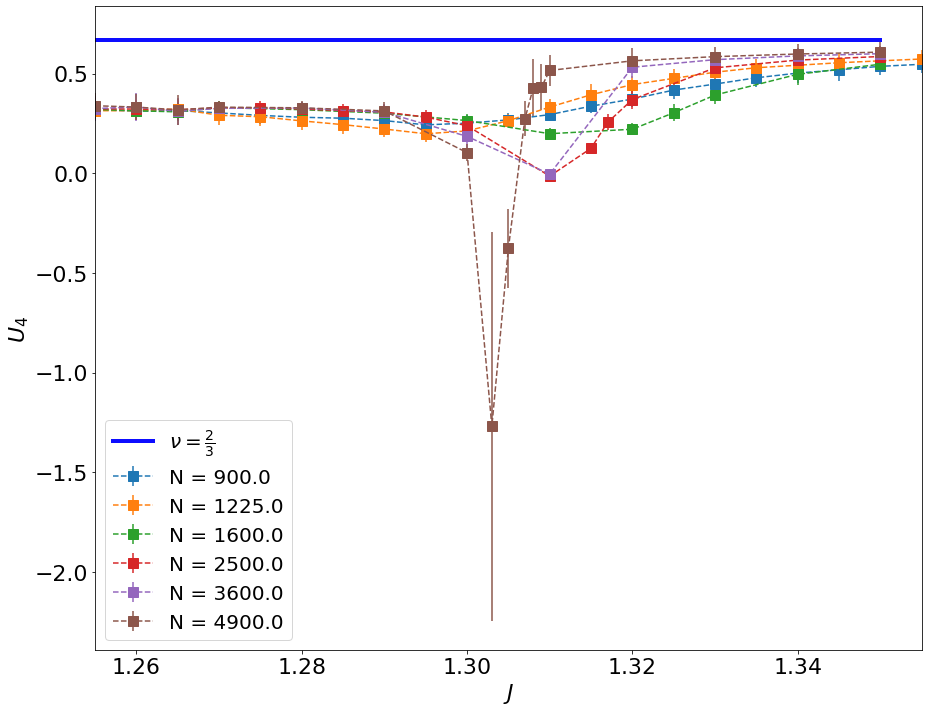
\includegraphics[width=\textwidth]{Images/bindercumulants_longchains.png}
		\caption{ Binder cumulant for long chains on the critical region}
		\label{fig:bcshort_longbc}
	\end{subfigure}
	\begin{subfigure}[b]{0.45\textwidth}
	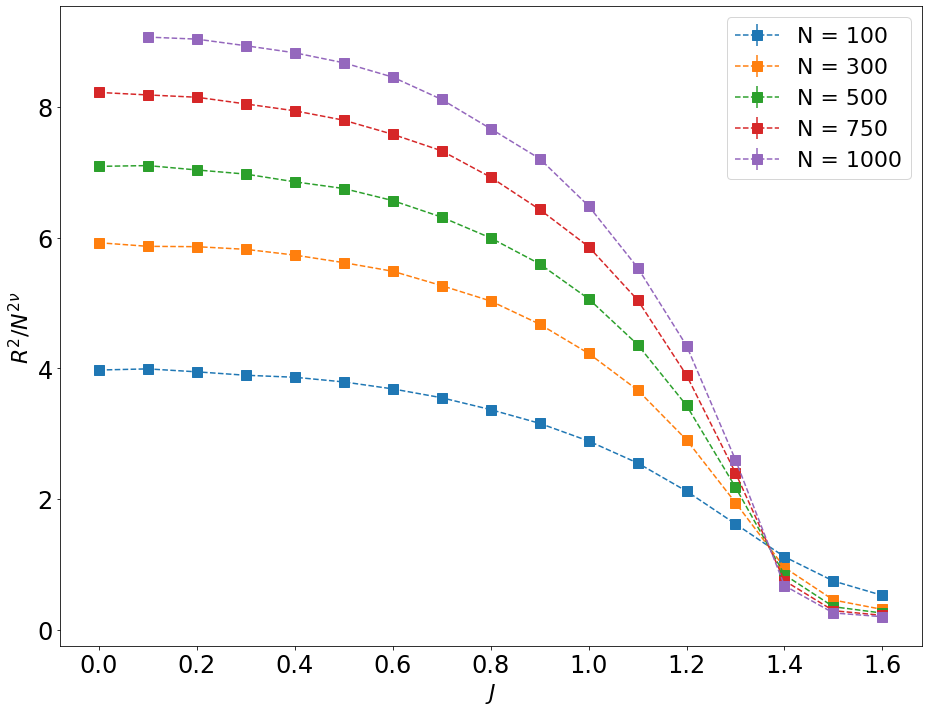
\includegraphics[width=\textwidth]{Images/rscaling_shortchains.png}
		\caption{ Scaled mean radius from simulations short chains   }
		\label{fig:bcshort_shortradius}
	\end{subfigure}
	\begin{subfigure}[b]{0.45\textwidth}
		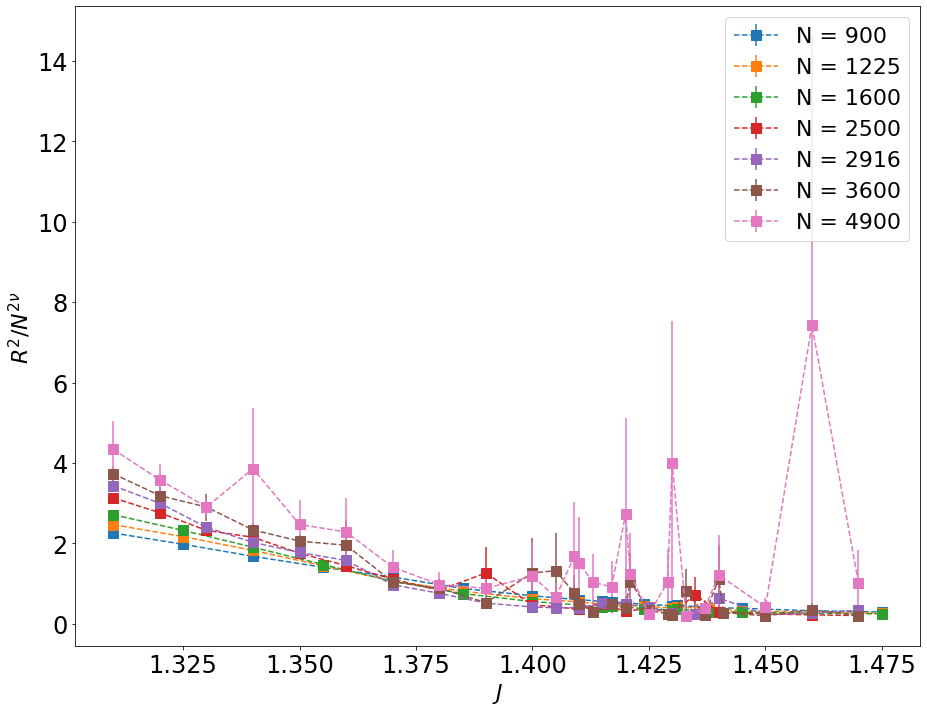
\includegraphics[width=\textwidth]{Images/rscaling_longchains.png}
		\caption{Scaled mean radius with zoom-in at the critical interval }
		\label{fig:bcshort_longradius}
	\end{subfigure}
	\caption{ Binder  cumulants \eqref{binderqum} and mean radius \eqref{endtoend} scaled by $\nu=\frac{4}{7}$.   }
	\label{fig:bcshort}
\end{figure}

\subsubsection{Magnetic phase transition} \label{sec:crossing}

We compute Binder cumulamts \eqref{binderqum} with the aim of determining  order of magnetic transition. 

The Binder cumulants (top Figure \ref{fig:bcshort_longbc}) has lower limiting value $U_4=\frac{1}{3}$ as $J\rightarrow 0$ which is in a good agreement with analytically obtained value in Section \ref{U4J0}. For large interaction energy  constant $J$, the system  signs ordering behavior, as expected, $U_4=\frac{2}{3}$. 


 Figure \ref{fig:bcshort_longbc} shows that Binder parameter curves does not diverge. Therefore, our computational results do not detect the first-order transition. Figure \ref{fig:U4_zoomin} illustrates cumulants in the narrow region where curves cross. %Following Ref. \cite{Hasenbusch_2008}, 
 Binder parameter are represented as a function of $1/N$ in figure Figure \ref{fig:U4_1N} varying $J$. The horizontal line should correspond the critical point. However, due to  large errobars and finite-size corrections, we cannot determine $J_cr$ place according to this plot. 

\begin{figure}
	\centering
	\captionsetup{justification=centering}
	\begin{subfigure}[b]{0.45\textwidth}
		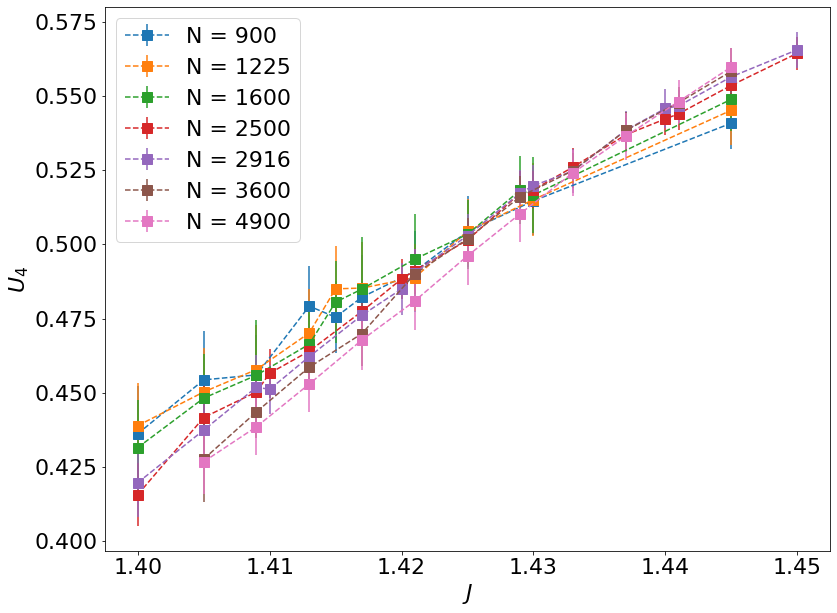
\includegraphics[width=\textwidth]{Images/bindercumulants_longchains_deep.png}
		\caption{Zoom-in of Figure \ref{fig:bcshort_longbc}.   }
		\label{fig:U4_zoomin}
	\end{subfigure}
	\begin{subfigure}[b]{0.45\textwidth}
		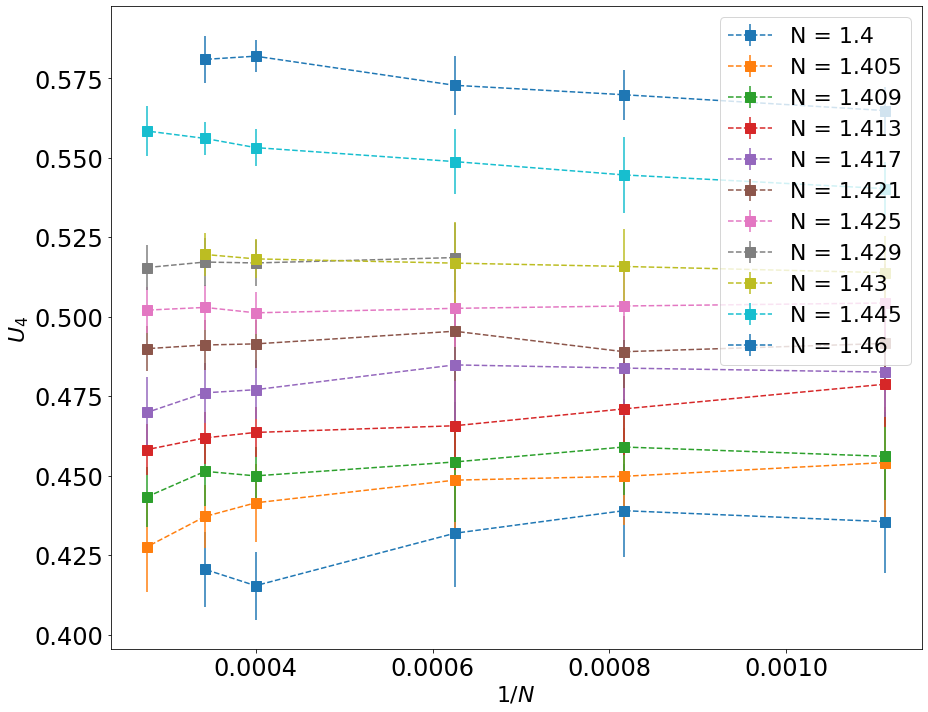
\includegraphics[width=\textwidth]{Images/bindercumulants_longchains_1n.png}
		\caption{Binder cumulants as a function of $1/N$ for a range of $J$. }
		\label{fig:U4_1N}
	\end{subfigure}
	\caption{ Binder cumulants at the critical region.  }
	\label{fig:U4}
\end{figure}



To estimate critical values for cumulants $U_4$ and phase transition point $J_{cr}$, we perform paired linear intersections. The procedure to analyze Monte-Carlo data is following: 

1. Choose the pair of two different N values for length of the chain. Choose the range of values for interaction energy J. This segment should be as short as possible and include the point of intersection of the two curves. 

2. We need to obtain the errors to estimated Binder cumulant. To that end, we use Gaussian sampling. 

For each point from the set generate $n_{samples}$ values using Normal distribution with mean and standard error of $\langle m^2 \rangle  $ and $\langle m^4 \rangle$ as parameters: $ M2_{J, N} \sim N (\langle m^2 \rangle  , \sigma (\langle m^2 \rangle  ))$, $ M4_{J, N} \sim N (\langle m^4 \rangle  , \sigma (\langle m^4 \rangle  ))$. We generate for each value $J$ 1000 samples. For each pair of sampled $m_2, m_4$ we calculate the Binder cumulant \eqref{binderqum}. 

3. Using generated set, for each pair $J$ and $N$ make estimation for mean and standard deviation $\langle U_4 \rangle$.

4. Now, we have  two curves of calculated $U_4$ with errorbars for two values of $N$. Apply weighted least squares regression to find crossing point. Save the obtained estimation for $\hat{J}$. 

5. Repeat steps 2-5 $n_{lines}$ times. We repeat it $n_{lines}=1000$ times. 

6. At the end, we have $n_{lines}$ of estimated $\hat{J}$ where two curves cross. 
 
 \begin{figure}[!ht]
	\centering
	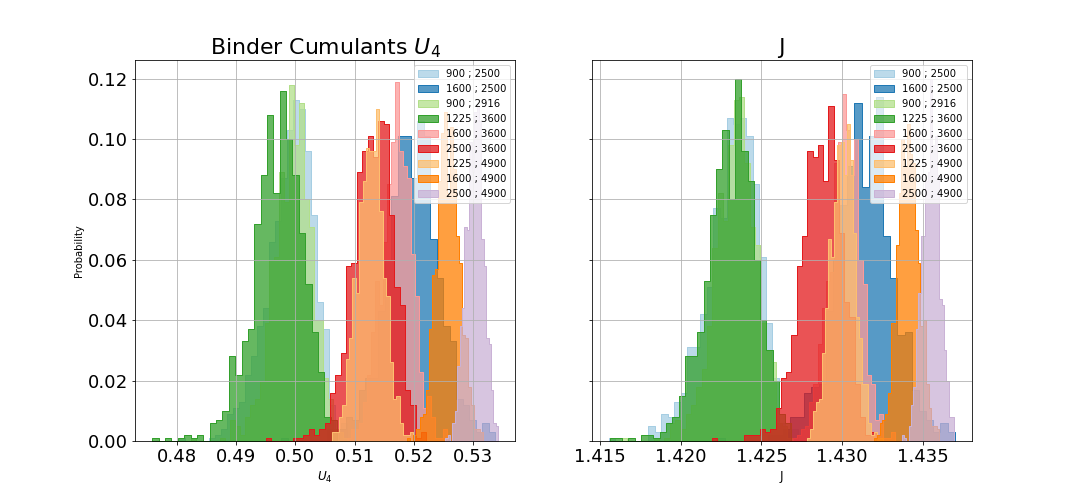
\includegraphics[scale=0.3628]{Images/bc_cov.png}
	\caption{$h=0$. Histograms of estimated $U_4$ and $J_{cr}$ from paired regressions.  }
	\label{fig:Jmagnethistogram}
\end{figure} 

 \begin{figure}[!ht]
	\centering
	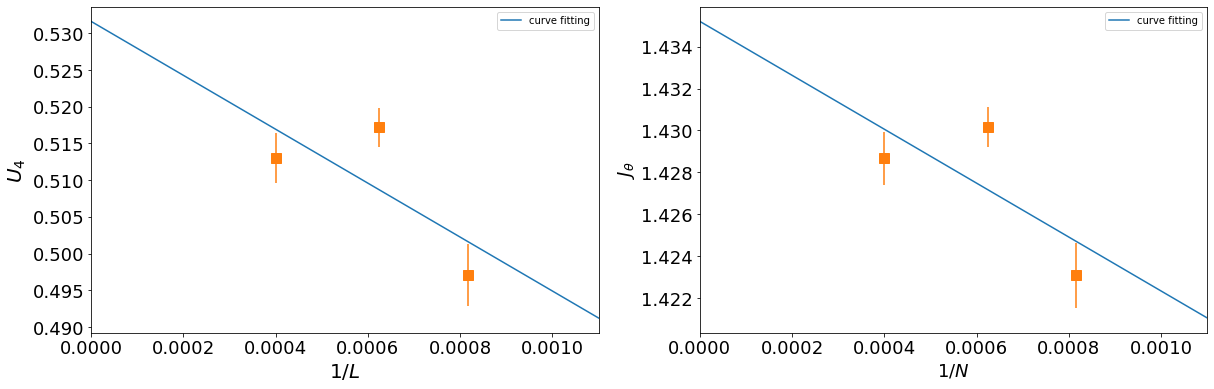
\includegraphics[scale=0.3628]{Images/criticalu4_4900.png}
	\caption{ Histograms of estimated $U_4$ and $J_{cr}$ from paired regressions with $N=3600$.  }
	\label{fig:JmagnetLinear}
\end{figure} 

Histograms for pairs from Figure \ref{fig:Jmagnethistogram} shows us how the size of systems affect the estimations $\hat{J}$. One way to choose the estimation for phase transition point $\hat{J}$ in thermodynamic limit is to focus on pairs for long chains with not too large errorbars. We choose $N=3600$. 

Consider the set of results for $N=3600$. We have calculations for four pairs $[N_i, 3600]$ which presented in Figure \ref{fig:Jmagnethistogram}. We construct the dependence of estimates $\hat{J_{\theta}}$ on $1/N_i$. Using this measurements, we perform curve-fitting using weighted least squares regression. The fitting results are plotted in Figure \ref{fig:JmagnetLinear}. Estimation of critical point is the point of the limit $1/N_i \rightarrow 0$. The errorbars are calculated using module $linregress$ from SciPy. We obtain the following results: 
\begin{equation}
\label{eq:critical_J_magnet_2D}
J_{cr}^{3600} \approx  1.43519999570142 \pm 0.0079203
\end{equation}
%Estimated value from the zero point: $J_{\theta} \approx 1.3(0)$.

The estimation of critical value of cumulant at the magnetic transition is following: $U_4 \approx 0.55(5) $. This value is far from the Binder cumulant  value for classical Ising model on the square lattice with periodic boundary condition and for Ising model on SAWs in 2D \cite{PhysRevE.104.054501}. 

Figure  \ref{fig:JmagnetLinear} shows that the Binder cumulant of crossing  points for $N=3600$ is increasing with using larger second chain size. The same dependence on system size was found in studying XY model on square lattice at  KT transition \cite{Hasenbusch_2008}.   

\subsubsection{ Estimation of $\hat{J_{\theta}}$} \label{sec:2DJthetatransition}

In the bottom of Figure \ref{fig:bcshort} we can see that scaled curves of mean radius for range of $N$ values cross approximately at the same point. To estimate the point of structural phase transition, we repeat the procedure with histograms for paired linear crossings described  in Section \ref{sec:crossing}, except for step 2. 
 
   \begin{figure}
 	\centering
 	\captionsetup{justification=centering}
 	\begin{subfigure}[b]{0.45\textwidth}
 		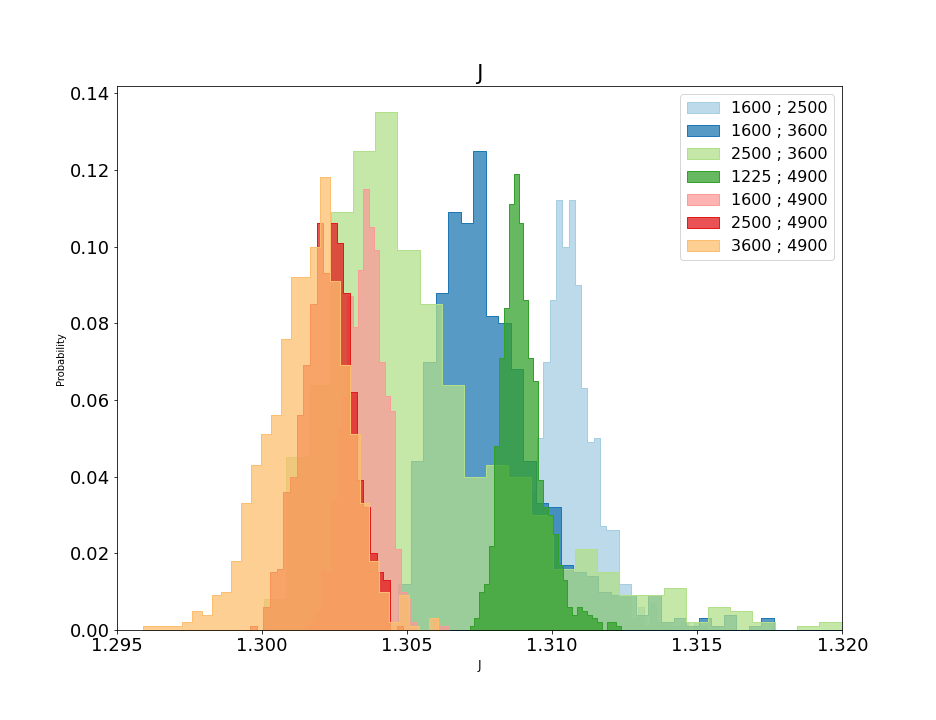
\includegraphics[width=\textwidth]{Images/radius_hist_cov.png}
 		\caption{ Histograms of estimated $J_{\theta}$ from paired regressions.  } 
 		\label{fig:Jthetahistogram}
 	\end{subfigure}
 	\begin{subfigure}[b]{0.45\textwidth}
 		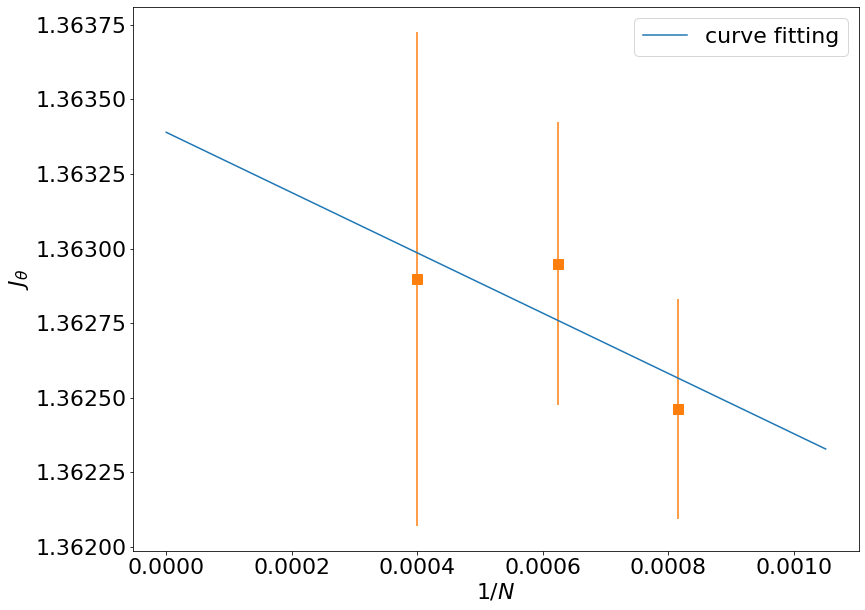
\includegraphics[width=\textwidth]{Images/criticalr2_4900.png}
 		\caption{  Crossing points using pairs with $N= 3600$. }
 		\label{fig:JthetaLinear}
 	\end{subfigure}
 	\caption{ Estimate for $J_{\theta}$ using pairs for $N=3600$.  }
 	\label{fig:JTheta}
 \end{figure} 
%Histograms for pairs from Figure \ref{fig:Jthetahistogram} shows us how the size of systems affect the estimations $\hat{J_{\theta}}$. One way to choose the estimation for phase transition point $\hat{J_{\theta}}$ in thermodynamic limit is to focus on pairs for long chains such as $N=3600$ and $N=4900$. Consider the set of results for $N=4900$. We have calculations for four pairs $[N_i, 4900]$ which presented in Figure \ref{fig:Jthetahistogram}. We construct the dependence of estimates $\hat{J_{\theta}}$ on $1/N_i$. Using this measurements, we perform curve-fitting using weighted least squares regression. The fitting results are plotted in Figure \ref{fig:JthetaLinear}. Estimation of critical point is the point of the limit $1/N_i \rightarrow 0$. We obtain the following results: 
%\begin{equation}
%\label{eq:critical_J_theta_2D}
%J_{\theta}^{3600} \approx 1.3(06); J_{\theta}^{4900} \approx 1.3(04).
%\end{equation}
%Estimated value from the zero point: $J_{\theta} \approx 1.3(0)$.

Repeating the linear fitting results Figure \ref{fig:JthetaLinear}, we obtained following estimated value from the zero point:
\begin{equation}
\label{eq:critical_J_theta_2D}
J_{\theta}^{3600} \approx  1.3633900514712 \pm 0.00050.
\end{equation}

 
  Our computational results shows that magnetic transition \eqref{eq:critical_J_magnet_2D} and structural transition \eqref{eq:critical_J_theta_2D} appears at the different points. The intervals within errobars do not overlap. Therefore, we cannot conclude that magnetic phase transition and structural transition happens at the same point, in contrast to Ising model on SAWs. Our MC the data is inconclusive, whether the transitions occur simultaneously or at distinct values of the coupling constant J. More work is needed to conclusively rule out one of possibilities.


 

\subsection{Distribution of $\langle cos \theta \rangle$ and $\langle e \rangle$ } \label{sec:distributions}
To study the phase transition order, we look to distributions of energy and magnetization.

%We start our observation of distributions with quite shore chain $N=1600$. Here (Figure \ref{fig:distributions}, top), we notice that energy distribution shape is getting wider around the critical region $J_{cr} \in [1.29; 1.32]$ which was defined using results from Figure \ref{fig:bcshort}. These curves  do not help enough to determine signs of first order transition. 

%Next, we turn our attention to the longer chains $N=2500$ (Figure \ref{fig:distributions}, medium). In this case, we see broad maybe-bimodal shape of energy distribution at the points $J=1.317$ and $J=1.32$.  

%Finally, we investigate the Monte-Carlo results for $N=4900$ (Figure \ref{fig:distributions}, bottom). The curve of the energy distribution obtained for simulation in $J=1.307$ is bimodal which corresponds to the first-order phase transition.   

  \begin{figure}
 	\centering
 	%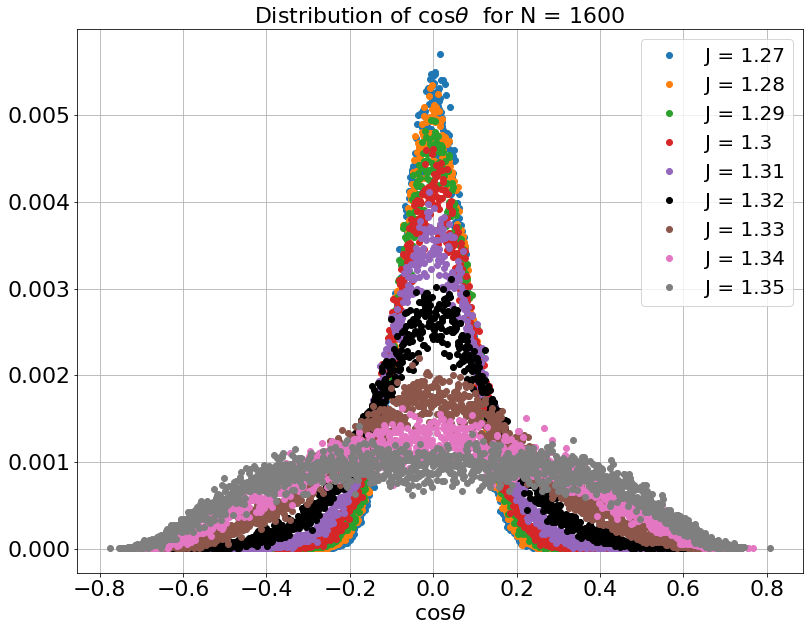
\includegraphics[scale=0.25]{Images/distr_cos_1600.png}
 	%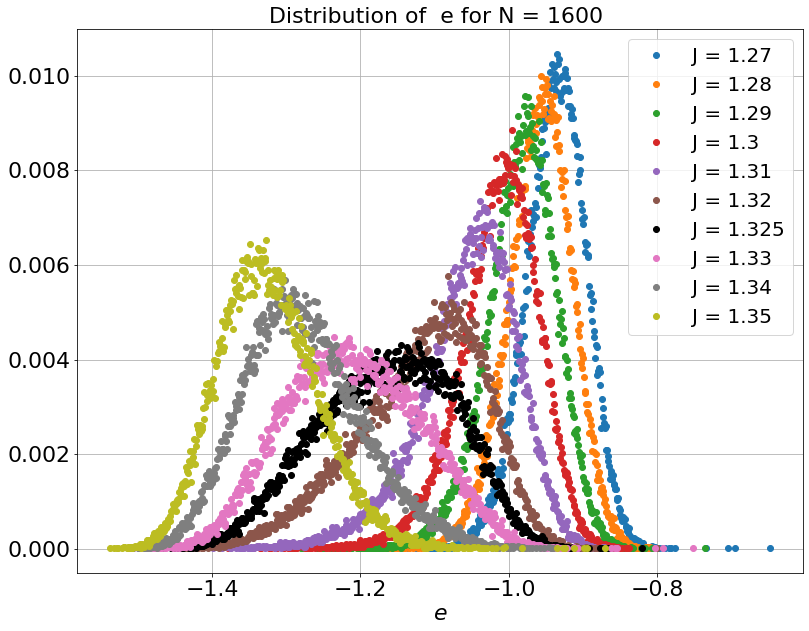
\includegraphics[scale=0.25]{Images/distr_energy_1600.png} \\
 	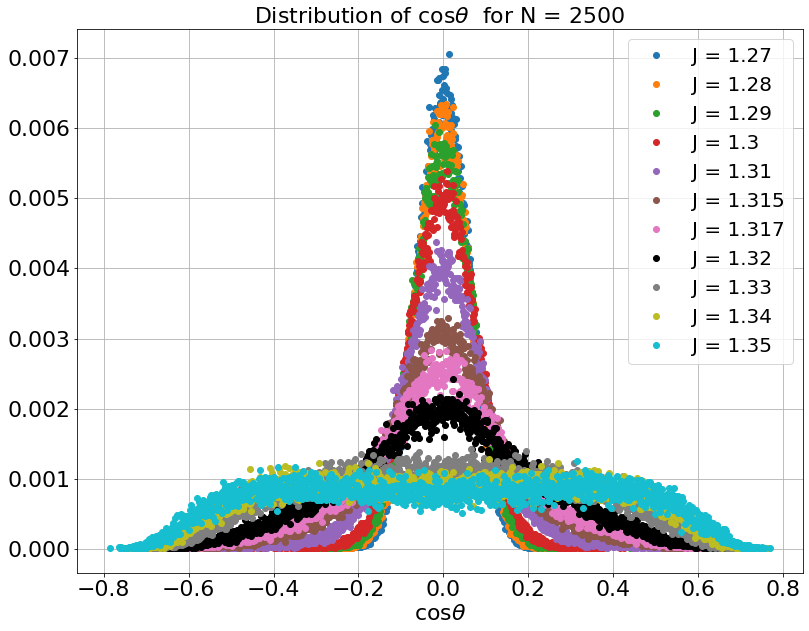
\includegraphics[scale=0.25]{Images/distr_cos_2500.png}
 	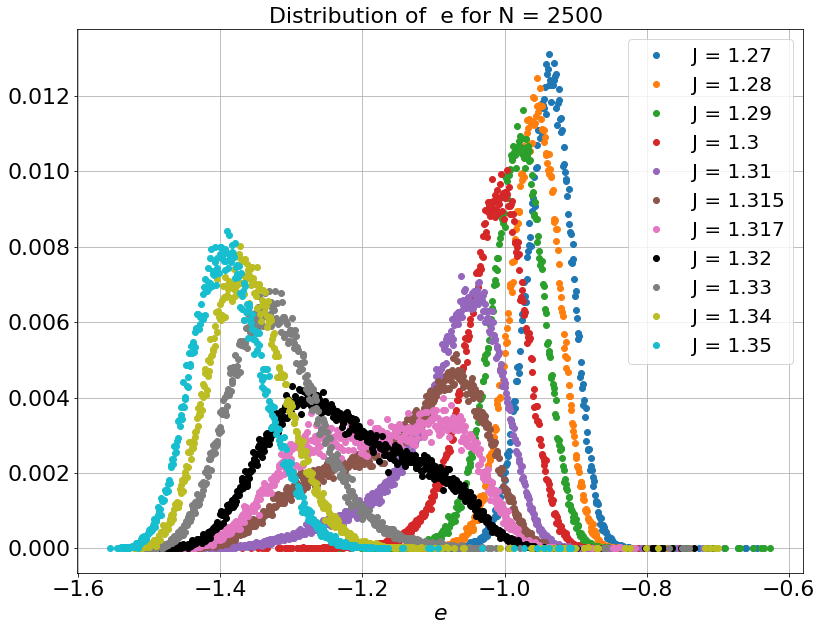
\includegraphics[scale=0.25]{Images/distr_energy_2500.png}
 	\\
 	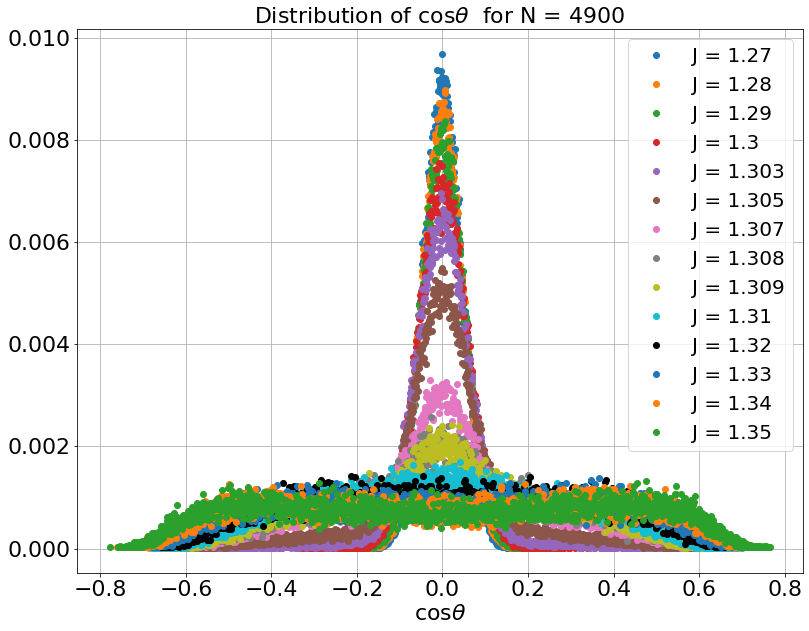
\includegraphics[scale=0.25]{Images/distr_cos_4900.png}
 	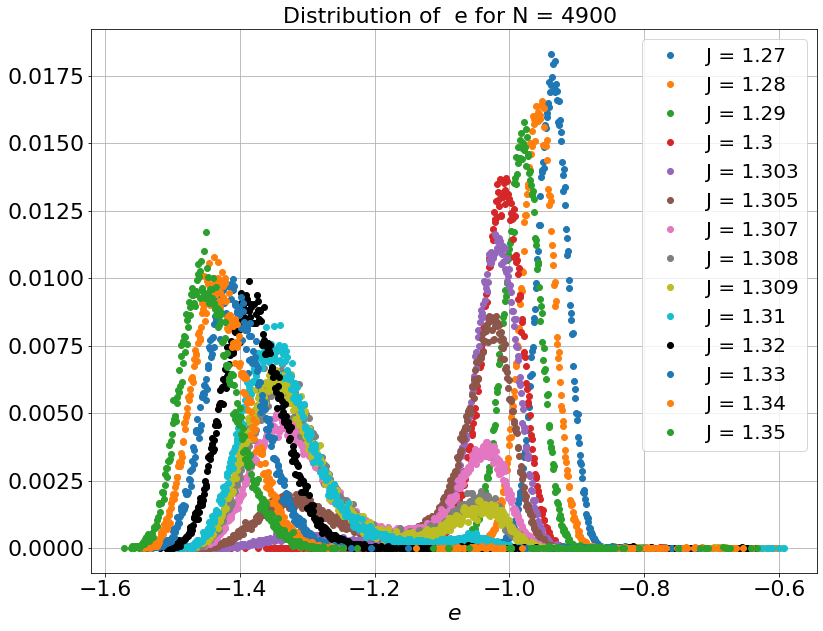
\includegraphics[scale=0.25]{Images/distr_energy_4900.png}
 	\caption{ Distributions for chains $N=2500$ and $N=4900$ for various $J$.    }
 	\label{fig:distributions}
 \end{figure}
%
%To examine that shape of the energy critical distribution is truly bimodal, we monitor the curve over simulation and fix four phase of the simulation in Figure \ref{fig:distributione4900}. We see that the results at the beginning are quite noisy, however, the data converge to bimodal shape. Here, we can make an estimation $J_{\theta} \approx 1.3(0)$ as we obtain bimodal plot at the point $J=1.307$. 
%
%
% \begin{figure}[H]
%	\centering
%	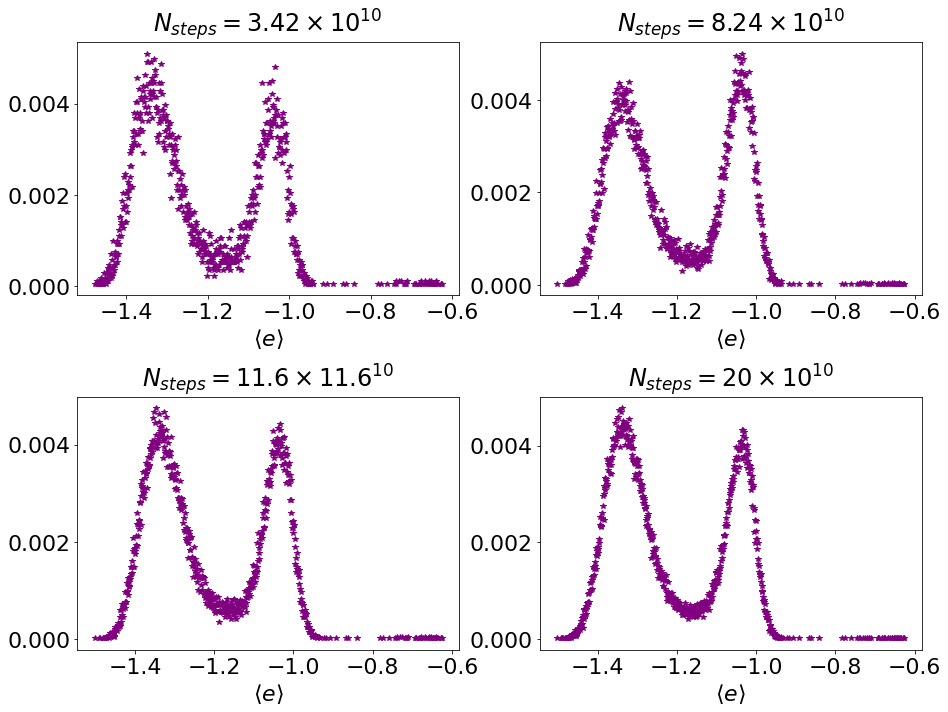
\includegraphics[scale=0.36]{Images/distr_energy_4900_time.png}
%	\caption{$h=0$.  }
%	\label{fig:distributione4900}
%\end{figure}

Figure \ref{fig:distributions} shows shapes of energy distribution across the structural transition \eqref{eq:critical_J_theta_2D} and magnetic transition  \eqref{eq:critical_J_magnet_2D}. The curves of distributions is Gaussian-like and do not sign any bimodal shapes. 

Additionally to energy, we consider mean $\cos \theta$ which represents a component of mean magnetization vector \eqref{meanmagnetization}. For points $J < J_{cr}$, curves of $\cos \theta$ distribution is similar to normal curve. Over the critical region, the shapes of distributions are far from Normal-like curves. Here we cannot conclude whether there is some signs of phase coexistence or not.  


%We notice that over the critical region the shapes of distributions are far from Normal-like curves and have signs of phase coexistence. \textbf{foster ?}

% \begin{figure}[H]
%	\centering
%	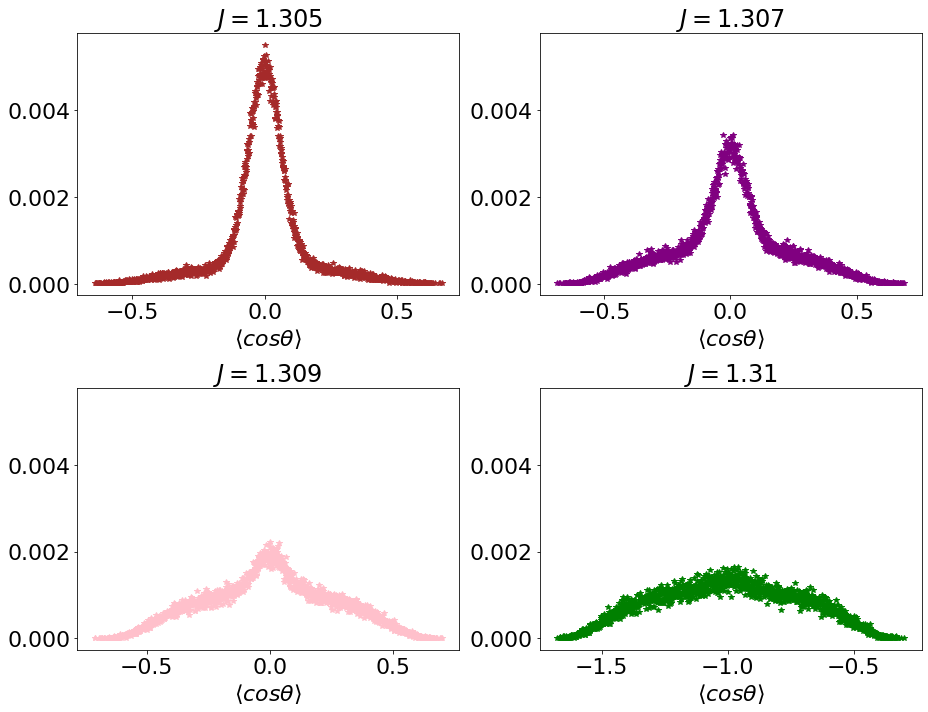
\includegraphics[scale=0.36]{Images/distr_cos_4900_J.png}
%	\caption{$h=0$.  }
%	\label{fig:distributioncos4900}
%\end{figure}


\subsection{Summary for 2D case}
We study XY model on self-avoiding walks on the square lattice (2D case) using Monte-Carlo simulations. In this work, we consider regime when both conformations and spins are dynamic. Obtained numerical result do not show signs of first-order transition.  We cannot conclude that magnetic phase transition \eqref{eq:critical_J_magnet_2D} and structural transition \eqref{eq:critical_J_theta_2D}  happens at the same region, in comparison to Ising model on SAWs. Our MC the data is inconclusive, whether the transitions occur simultaneously or at distinct values of the coupling constant J. More work is needed to conclusively rule out one of possibilities.


\section{XY model on SAWs, 3D}
Here, we study XY-model on SAWs on the cubic lattice. The sequence of our actions is similar to investigation of 2D case. 

In this section, we consider short chains up to $N=700$ which is much shorter than we study for 2D case. The reason of it is the lattice implementation which requires to keep $2dN^3=6N^3$ nodes in the memory.

We make short MCMC simulations for short chains from $N=50$ to $N=300$ to narrow the region of critical behavior. MC steps. We use following values for update probabilities: $P_{local}=0.6$, $P_{reconnect}=0.499$, $P_{Wolff}=0.001$. For $N=300$, we run at least $1.6 \times  10^{9} $ algorithm iterations.

For longer chains from $N=400$ to $N=700$ we use these values for update probabilities in the algorithm: $P_{local}=0.5$, $P_{reconnect}=0.4$, $P_{Wolff}=0.1$. We run at least $ 8 \times 10^{10}$ MC steps for $N=700$.

In all runs, we skip first $ 400 \times N^2$ MC iterations as the system should achieve equilibrium. We save each $1000$th sample to compute properties. 

\subsection{Thermodynamic properties}

 First, we measure the mean square magnetization \eqref{secondmomentmagnetization} and the mean energy \eqref{hamiltonian} to  study the system. 
 \begin{figure}
	\centering
	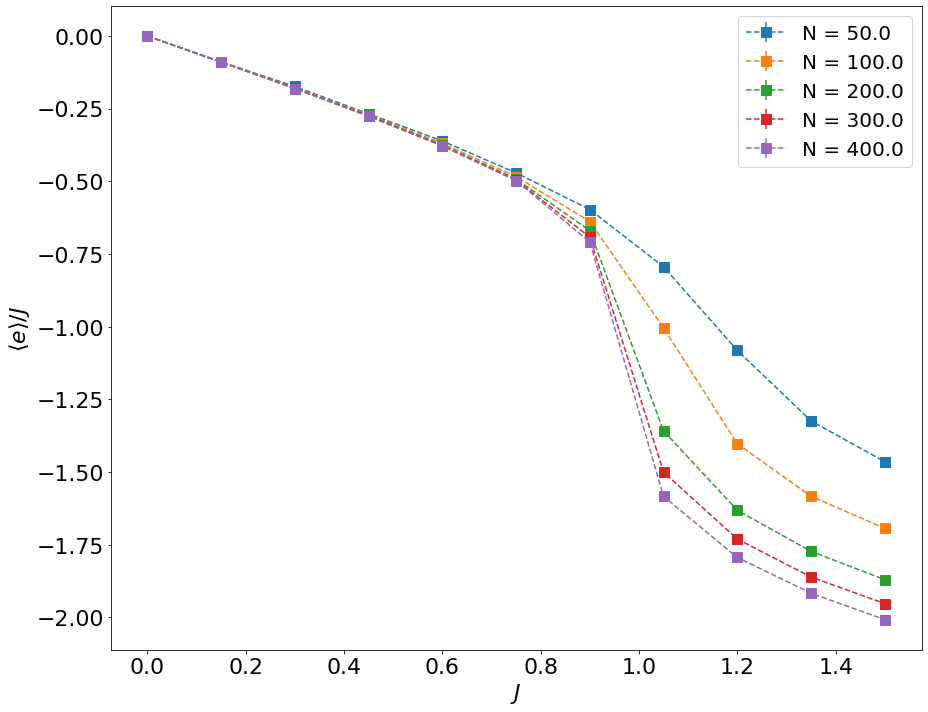
\includegraphics[scale=0.23]{Images/3_energy_shortchains.png}
	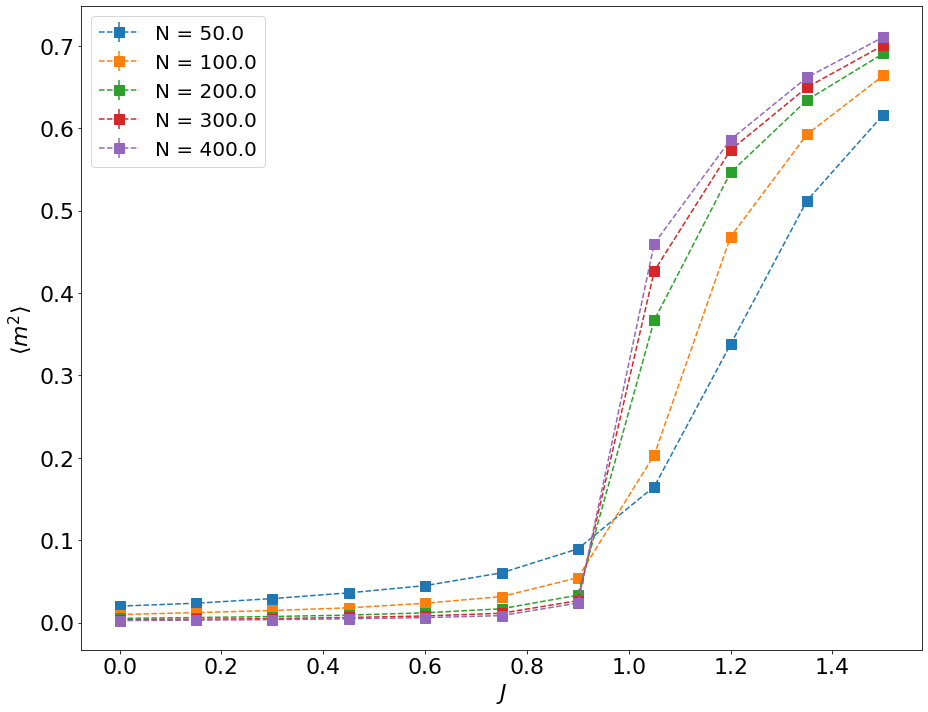
\includegraphics[scale=0.23]{Images/3_magnetization2_shortchains.png} \\
	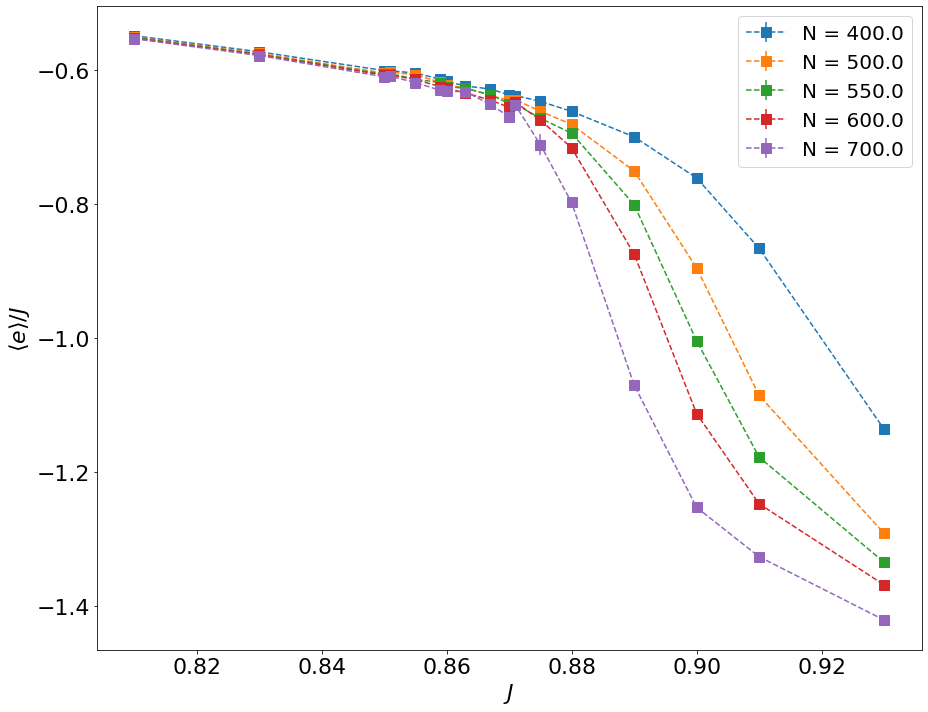
\includegraphics[scale=0.23]{Images/3_energy_longchains.png}
	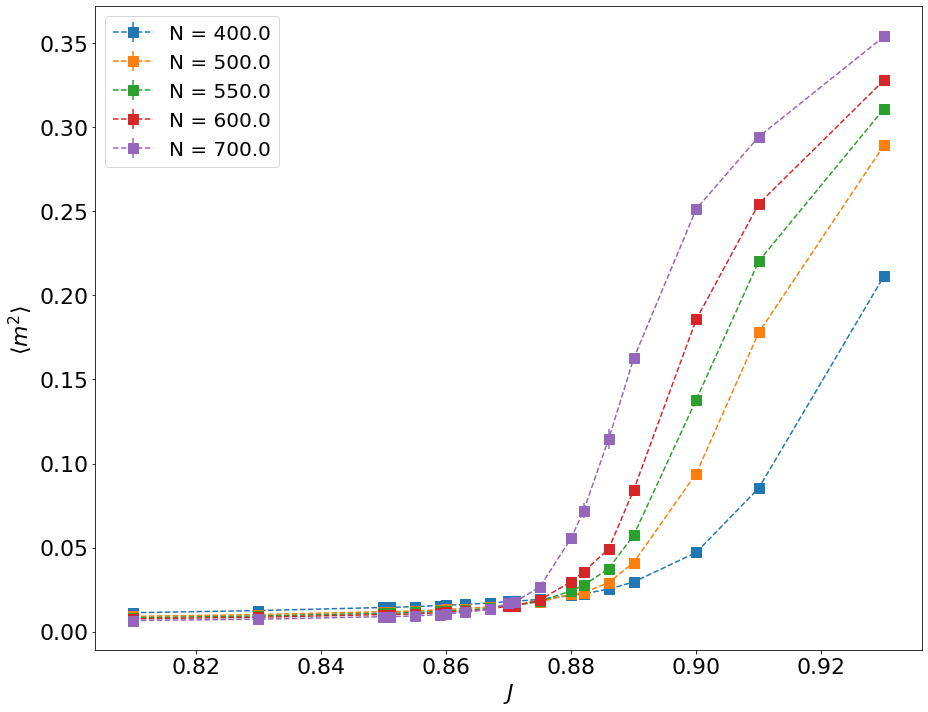
\includegraphics[scale=0.23]{Images/3_magnetization2_longchains.png}
	\caption{$h=0$. Mean energy \eqref{hamiltonian} and   second moment of magnetization \eqref{secondmomentmagnetization}. }
	\label{fig:energymagshort_3D}
\end{figure}

The squared magnetization (right column in Figure \ref{fig:energymagshort_3D} ) grows as the interaction energy $J$ increases. This behavior is similar to 2D case. 

The mean energy (left column in Figure \ref{fig:energymagshort_3D} )  rapidly decreases for low-temperature regime which could be a sign of compact ordered phase. 

From curves of both properties mean squared magnetization and mean energy, we can expect that the critical point is in the interval $J_{\theta} \in [0.84; 0.92]$.

\subsection{Structural properties}

Here we use the procedure from Section \ref{structureprocedure} to test the hypothesis that the critical exponent $\nu$ takes the proposed critical value \eqref{eq:nu_3D_Jtheta_flory} at the approximated critical region $J_{\theta} \in [0.84; 0.92]$. 

 \begin{figure}
	\centering
	\captionsetup{justification=centering}
	\begin{subfigure}[b]{0.45\textwidth}
		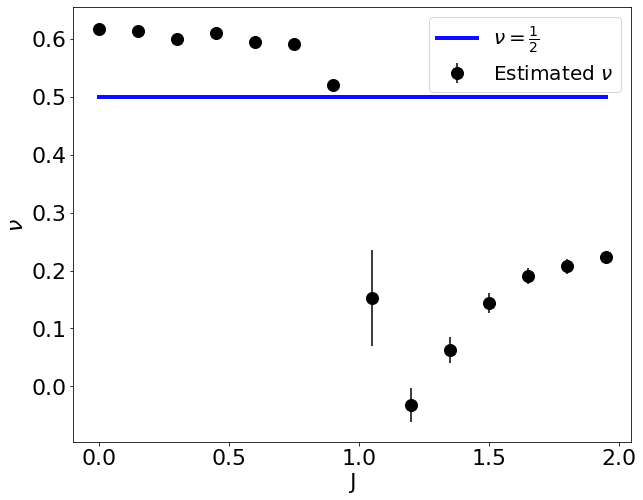
\includegraphics[scale=0.36]{Images/3_nu_shortchains.png}
		\centering{\caption{ From $N=50$ to $N=400$. } }
		\label{fig:nushort3D_short}
	\end{subfigure}
	\begin{subfigure}[b]{0.45\textwidth}
		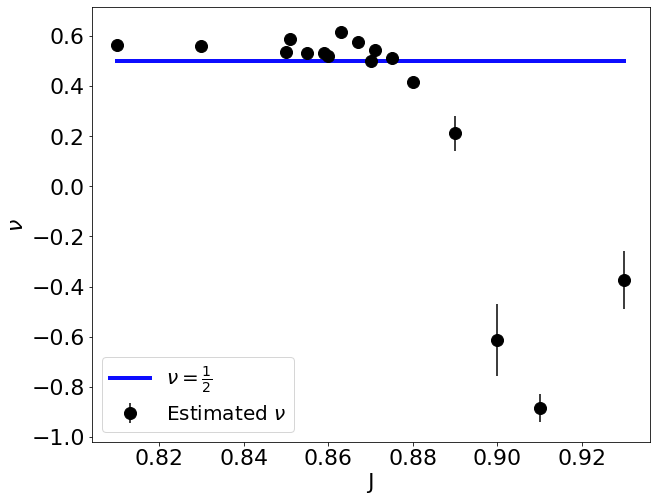
\includegraphics[scale=0.36]{Images/3_nu_shortchains_deep.png}
		\caption{ From $N=400$ to $N=700$. }
		\label{fig:nushort3D_long}
	\end{subfigure}
	\caption{$h=0$. Estimates with errorbars of critical exponent $\nu$ .   }
	\label{fig:nushort3D}
\end{figure}
Figure \ref{fig:nushort3D} illustrates the obtained results for $\nu$ estimations. In the non-interacting regime $J=0$, we get $\nu \approx 0.6(1) $ for the short chains from $N=50$ to $N=400$. This result is close to Flory prediction \eqref{eq:nu_3D_J0_flory}. We also see that the possible critical value \eqref{eq:nu_3D_Jtheta_flory} appears approximately at the region $J_{\theta} \in [0.87; 0.89]$.  

 \begin{figure} 
	\centering
	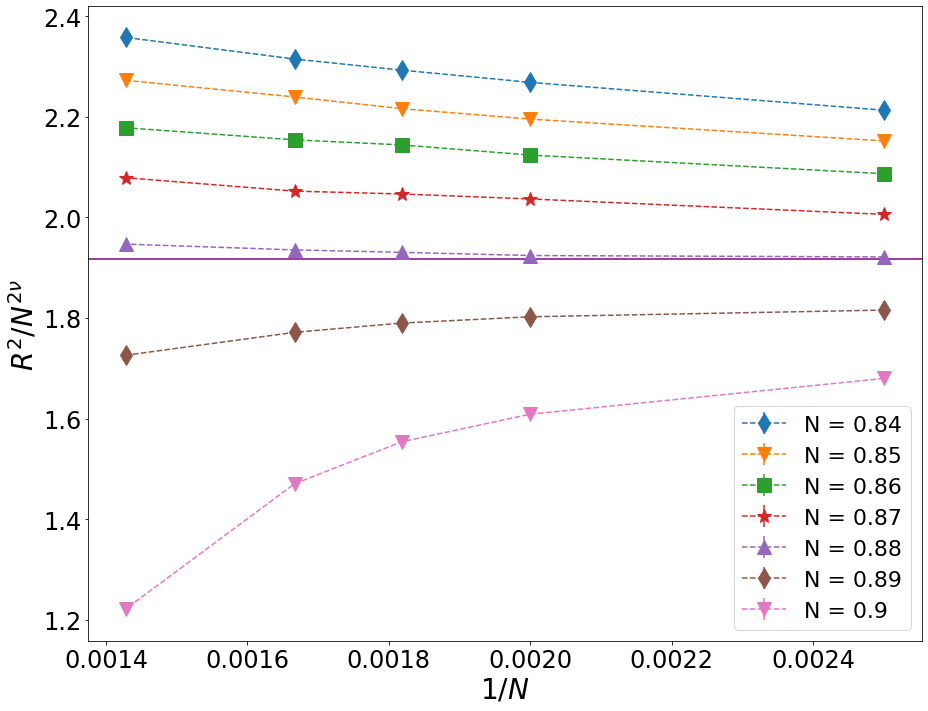
\includegraphics[scale=0.22]{Images/rscaling_longchainscross_3D.png} 
	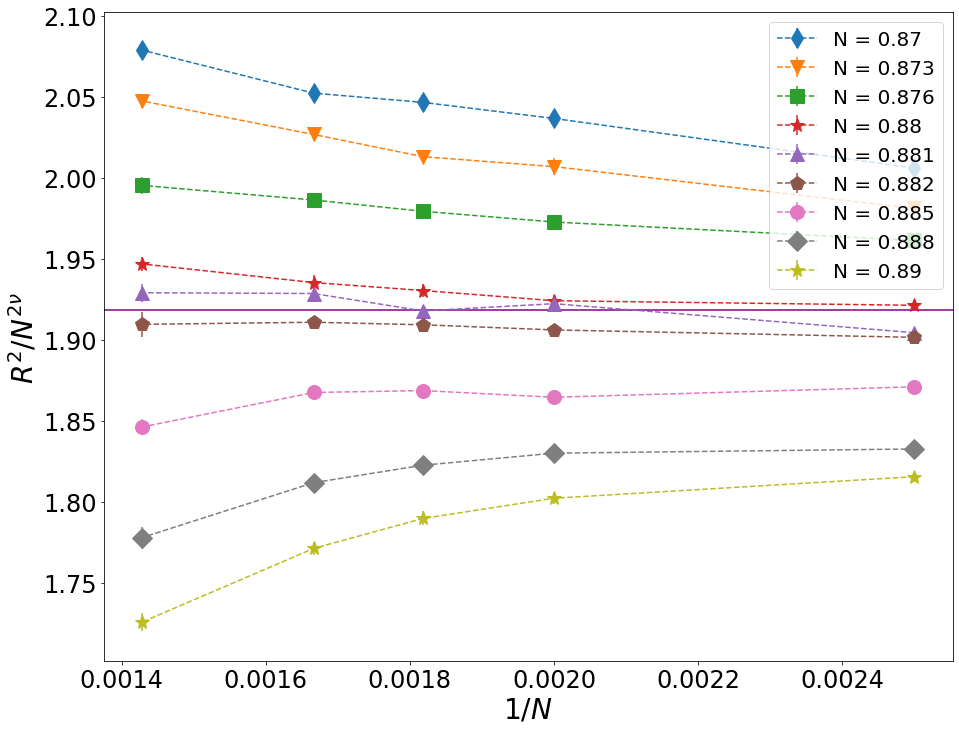
\includegraphics[scale=0.22]{Images/rscaling_longchainscross_3D_deep.png} 
	\caption{  Scaled Mean-squared end-to-end distance using $\nu_{\theta}=1/2$ as a function of $1/N$ from $N=400$ to $N=700$.  The solid  purple horizontal line corresponds to structural phase transition and placed at the estimation from Section \ref{Transition_3D}.  }
	\label{fig:Rscaled3D}
\end{figure}

Figure \ref{fig:Rscaled3D} shows the scaled
mean-squared end-to-end distance by $\nu=1/2$ as a function of the chain length
$1/N$for a range of $J$. The horizontal line is expected to represent the point of structural phase transition and corresponds to the critical exponent $\nu_{\theta}$. As the left part of the plot matches longer chains, we assume that the scaled curve of the mean radius at  $\theta$-point should be horizontal more at the left part. We place the horizontal line at the estimated value where scaled curves cross using histogram procedure. The horizontal line is limited by red star-marked curve ($J=0.88$)  and pink circle-marked curve ($J=0.885$).  Therefore, according our calculations for chains up to $N=700$, the system undergoes the structural phase $J \in [0.88;0.885] $ with the critical exponent $\nu_{\theta} = \frac{1}{2}$. However, this visual inspection is not very reliable due to finite size effect.  %We use $\nu_{\theta} = \frac{1}{2}$ as the critical exponent for the further study. 

For further study, we note the critical exponent value $\nu_{\theta} = \frac{1}{2}$ and use it in the following section to scale mean radius. 


\subsection{Transition}\label{Transition_3D}

To investigate the critical behavior at the phase transition, we again calculate  the Binder cumulants values \eqref{binderqum} and scaled mean end-to-end distance  \eqref{endtoend}.
 \begin{figure}
	\centering
	\captionsetup{justification=centering}
	\begin{subfigure}[b]{0.45\textwidth}
		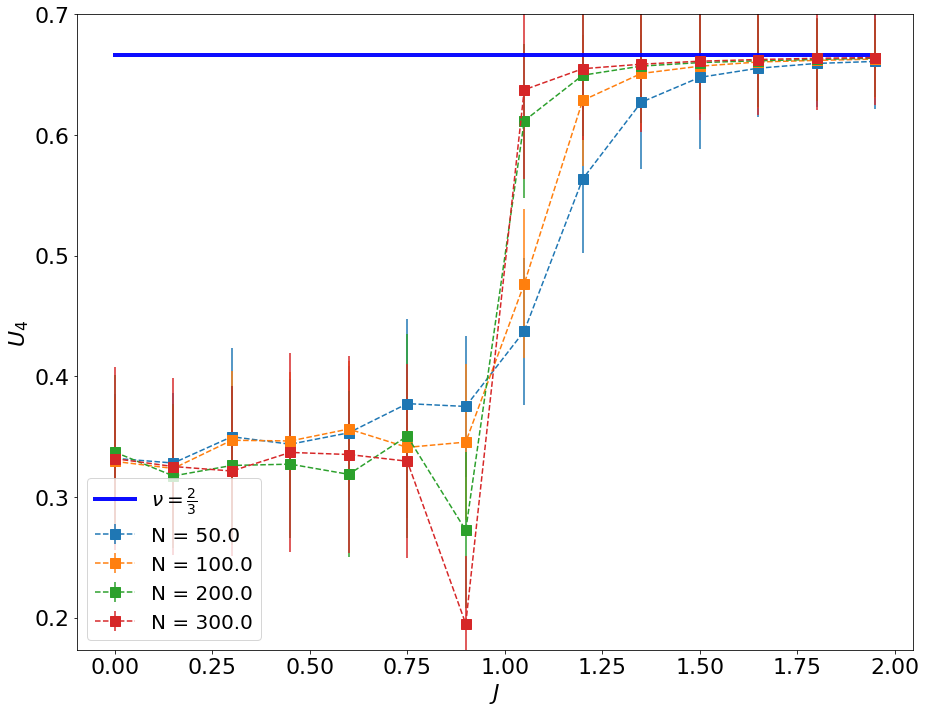
\includegraphics[width=\textwidth]{Images/3_bindercumulants_shortchains.png}
		\caption{Binder cumulant on the wide range of J with both lower and upper limits. }
		\label{fig:bcshort_shortbc_3}
	\end{subfigure}
	\begin{subfigure}[b]{0.45\textwidth}
		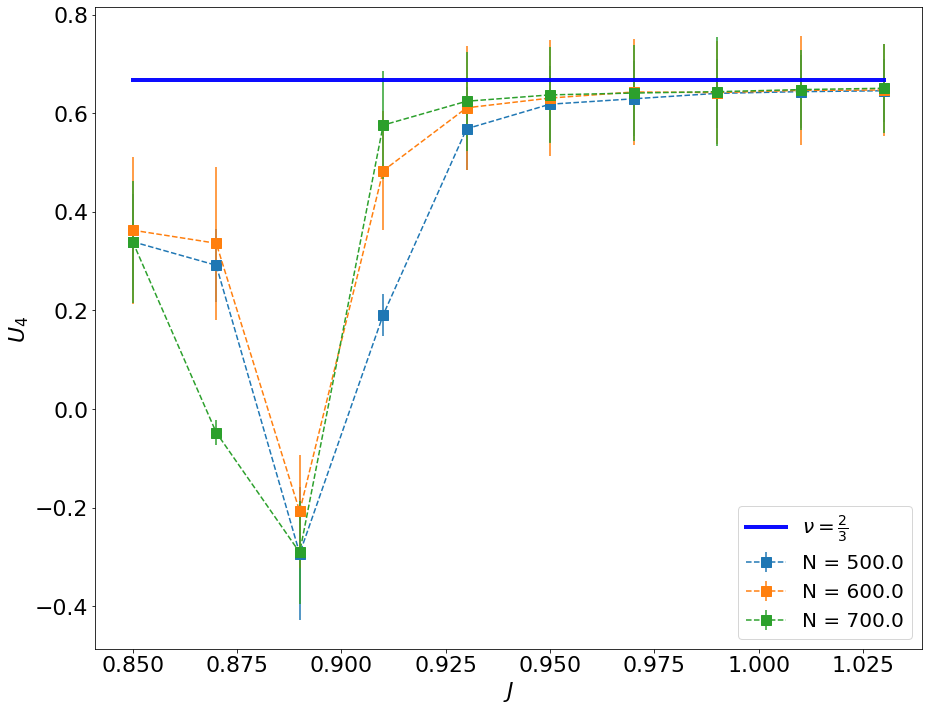
\includegraphics[width=\textwidth]{Images/3_bindercumulants_longchains.png}
		\caption{Binder cumulant on the interval including magnet phase transition.}
		\label{fig:bcshort_longbc_3}
	\end{subfigure}


	\begin{subfigure}[b]{0.45\textwidth}
		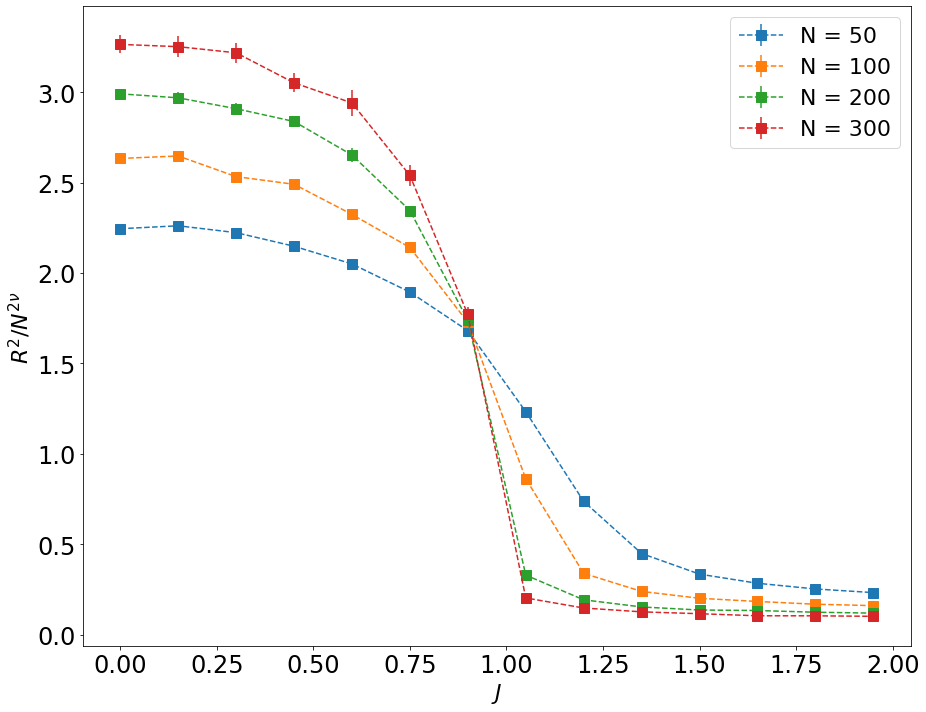
\includegraphics[width=\textwidth]{Images/3_rscaling_shortchains.png}
		\caption{ Scaled mean radius for short chains on the large range of J.  }
		\label{fig:bcshort_shortradius_3}
	\end{subfigure}
	\begin{subfigure}[b]{0.45\textwidth}
		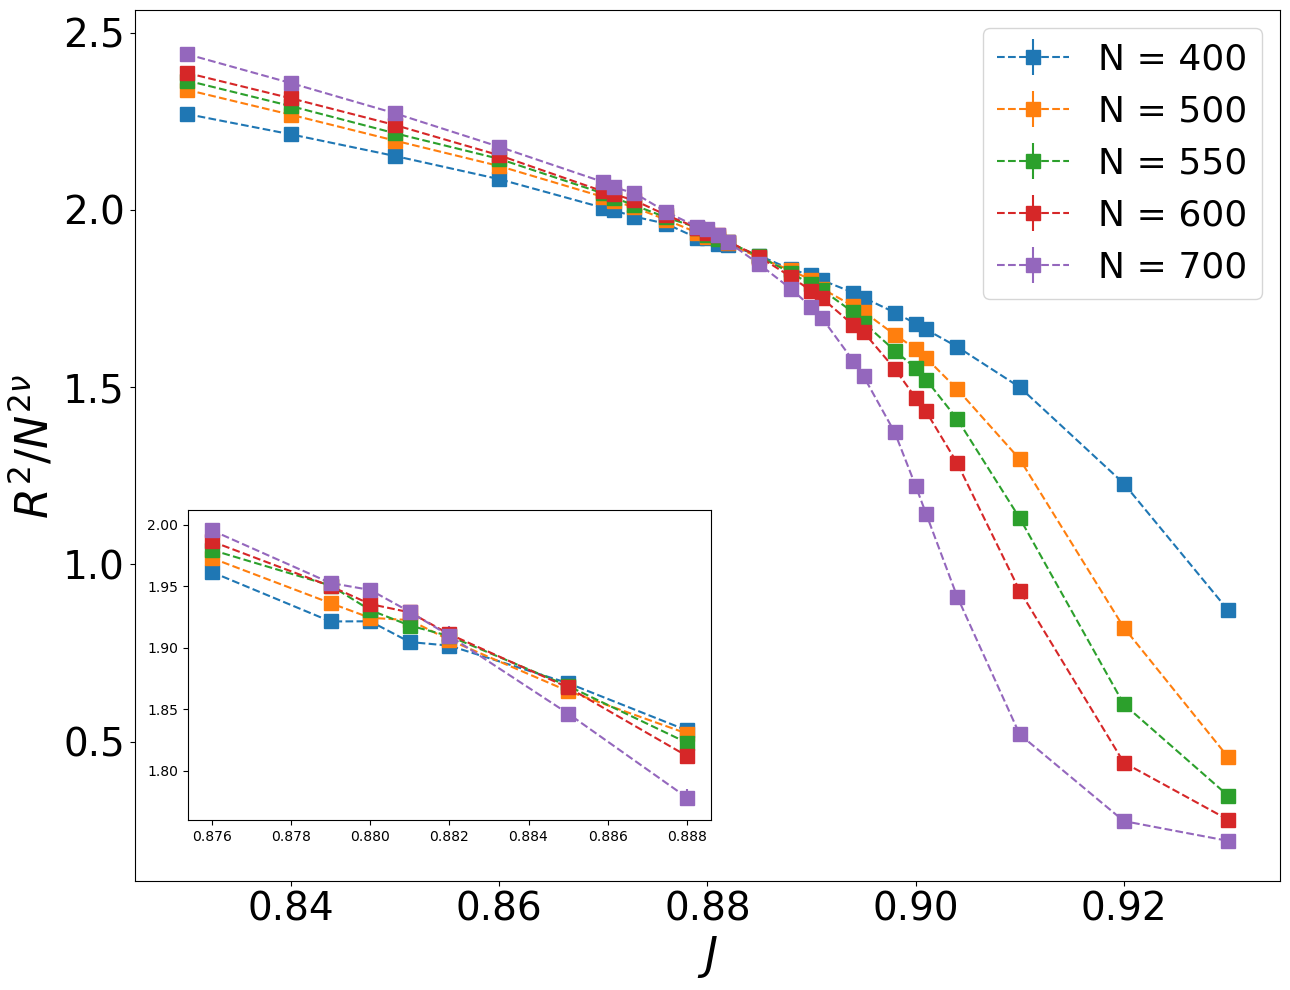
\includegraphics[width=\textwidth]{Images/3_rscaling_longchains.png}
		\caption{Scaled mean radius for long chains on the region with structural phase transition. }
		\label{fig:bcshort_longradius_3}
	\end{subfigure}
	\caption{$h=0$. Binder  cumulants \eqref{binderqum} and mean radius \eqref{endtoend}. The mean radius is scaled by $\nu = \frac{1}{2}$.   }
	\label{fig:bcshort_3D}
\end{figure}
As predicted in Section \ref{U4J0}, the Binder parameters (top Figure \ref{fig:bcshort_3D}) has lower limiting value $U_4=\frac{1}{3}$ as $J\rightarrow0$. For large values of coupling constant $J$, the system gets the ordering phase, for which $U_4=\frac{2}{3}$. 
    
Cumulant curves  diverges at the critical region. This is sign of the first-order phase transition \cite{PhysRevB.30.1477}. The similar results for diverged cumulants were obtained for Ising model on SAWs for 3D case \cite{PhysRevE.104.024122}.

 We check the distributions of thermodynamic characteristics in subsection \ref{sec:distributions_3D} to check whether energy distribution is bimodal and magnetic distribution show signs of phase coexistence. 


\subsubsection{ Estimation of $\hat{J_{\theta}}$}
 We can estimate the critical value of the interaction energy $J$ repeating the procedure described in the \ref{section:Transition}. Figure \ref{fig:Jthetahistogram_3D} shows us histograms for paired crosses. 


  \begin{figure}
	\centering
	\captionsetup{justification=centering}
	\begin{subfigure}[b]{0.45\textwidth}
		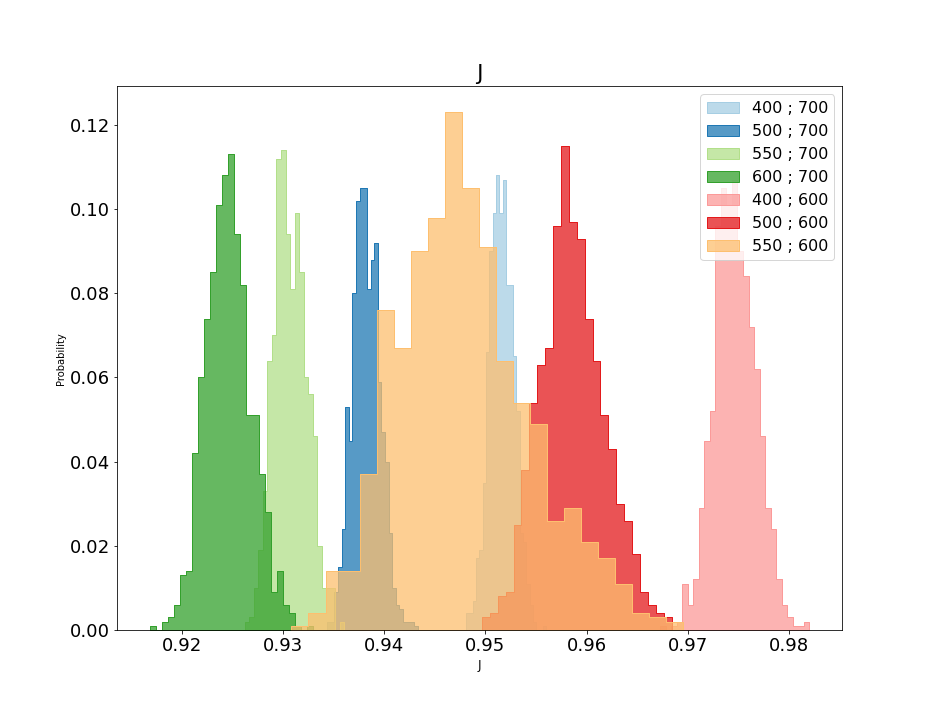
\includegraphics[width=\textwidth]{Images/radius_hist_cov_3D.png}
		\caption{ Histograms of estimated $J_{\theta}$ from paired regressions.    } 
		\label{fig:Jthetahistogram_3D}
	\end{subfigure}
	\begin{subfigure}[b]{0.45\textwidth}
		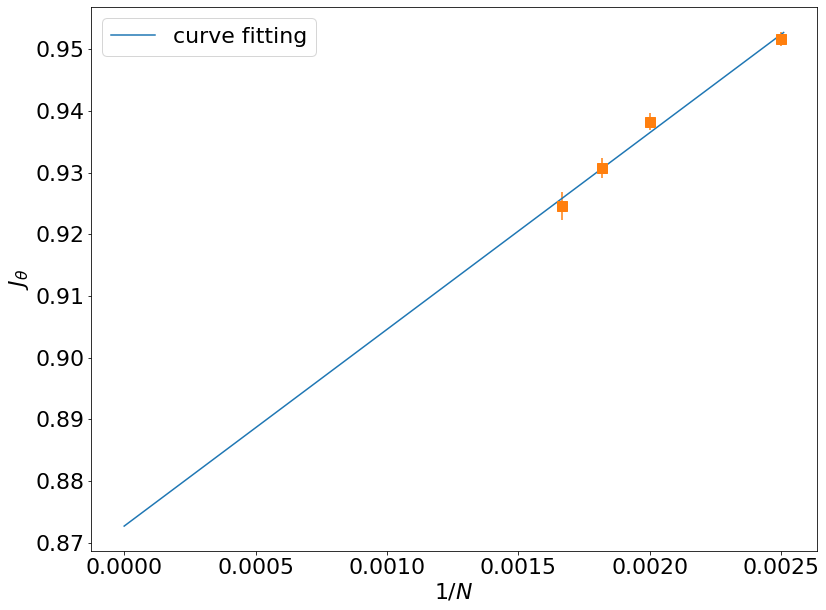
\includegraphics[width=\textwidth]{Images/criticalr2_3D.png}
		\caption{  Pairs with $N=700$. }
		\label{fig:JthetaLinear_3D}
	\end{subfigure}
	\caption{$h=0$. Estimate for $J_{\theta}$  }
	\label{fig:ThetaEsrimation_3D}
\end{figure}


The fitting results are plotted in Figure \ref{fig:JthetaLinear_3D}. Estimation of critical point is the point of the limit $1/N_i \rightarrow 0$. We obtain the following value: 
\begin{equation}
\label{eq:critical_J_theta_3D}
J_{\theta}^{700} \approx 0.876(5) .   
\end{equation}
 

\subsection{Distribution of $\langle cos \theta \rangle$ and $\langle e \rangle$ } \label{sec:distributions_3D}

In the subsection \ref{Transition_3D} we concluded that XY model on SAWs has first-order phase transition according to the divergence of the Binder cumulants. Now we look at the distributions of the energy and magnetization to study it further. 
 
  \begin{figure}
 	\centering
 	\captionsetup{justification=centering}
 	\begin{subfigure}[b]{0.45\textwidth}
 		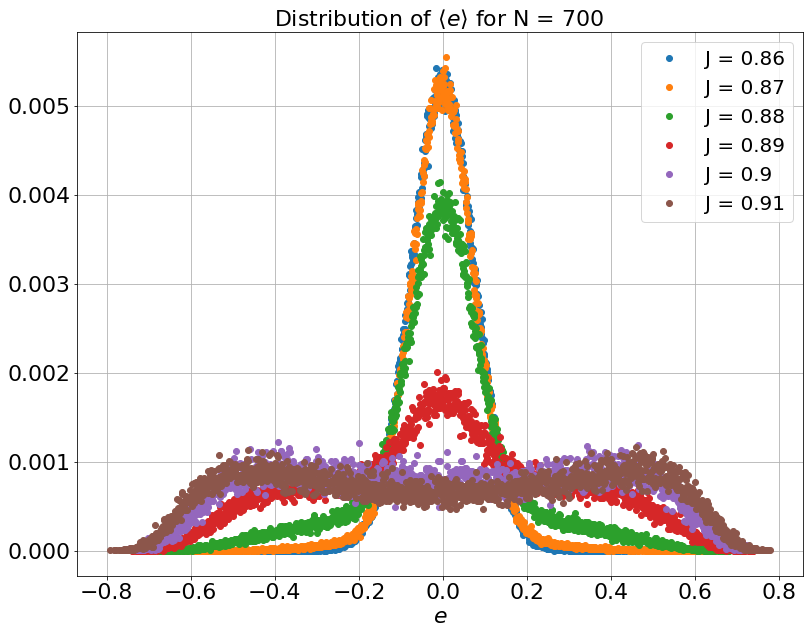
\includegraphics[width=\textwidth]{Images/distr_cos_700.png}
 		\centering{\caption{ The mean component $\cos \theta$ of magnetization vector.   } }
 		\label{fig:Distributions_3D_cos}
 	\end{subfigure}
 	\begin{subfigure}[b]{0.45\textwidth}
 		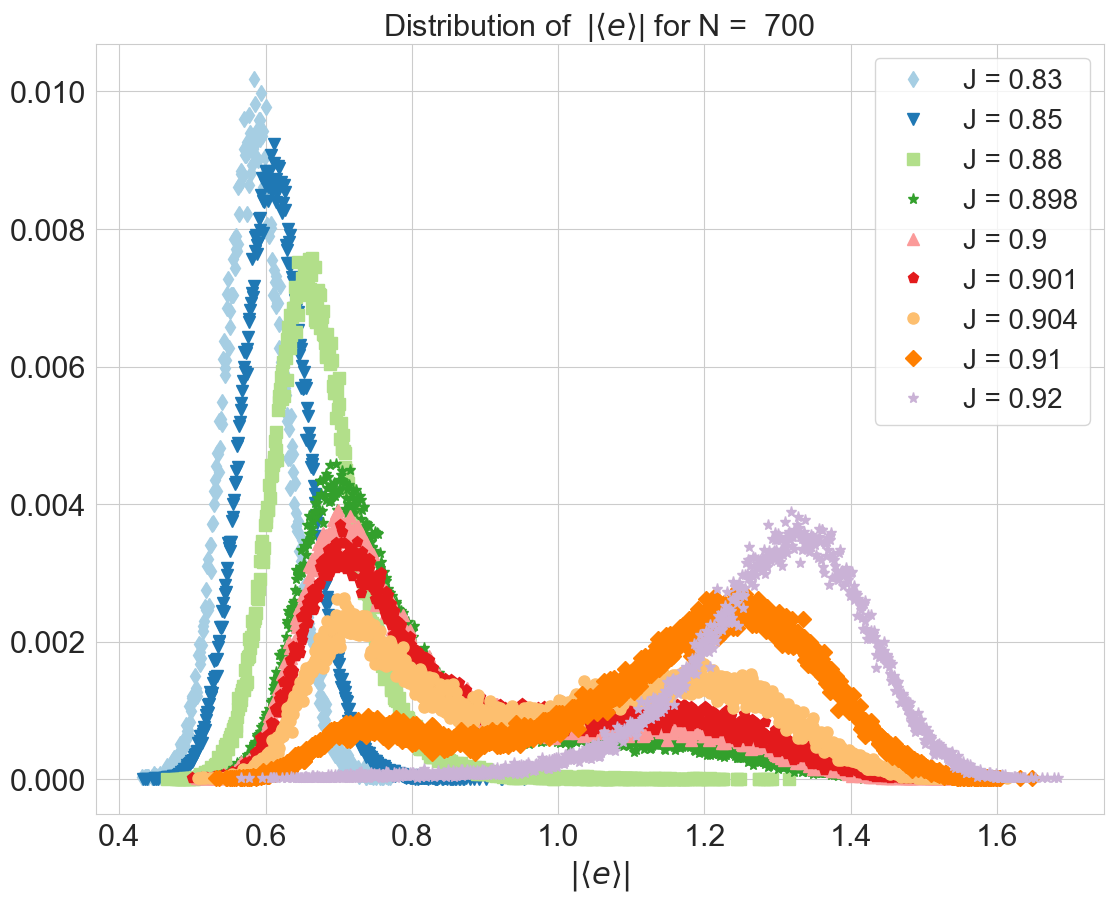
\includegraphics[width=\textwidth]{Images/distr_energy_700.png}
 		\caption{ The mean energy.  }
 		\label{fig:Distributions_3D_energy}
 	\end{subfigure}
 	\caption{ Distributions for chain $N=700$ for various $J$.  }
 	\label{fig:Distributions_3D}
 \end{figure}

Figure \ref{fig:Distributions_3D_energy} illustrates that energy distribution has bimodal shape approximately at $J \approx 0.904$. However, this region of bimodal curve is quite far ($\approx 0.03$) from the estimation for point of the structural transition \eqref{eq:critical_J_theta_3D} and the divergence region of minimum Binder cumulant (see Figure \ref{fig:bcshort_shortbc_3}). This could be caused by finite size effect as chains up to $N=700$ are not too long. 

We consider mean $\cos \theta$ which is a component of mean magnetization vector \eqref{meanmagnetization}. For points $J < J_{cr}$ before magnetic transition
transition, curves of $\cos \theta$ distribution is similar to normal curve which
is expected as this case corresponds to the sampling from uniform distribution $U \sim [-1;1]$ and convergence to the Gaussian.Over the critical region, the shapes of distributions are far from Normal-like curves. 

\subsection{Summary for 3D case}
 In this section, we present our computational results for XY model on cubic lattice. We simulated chains up to $N=700$ to study system at the transition region. Our computational data indicates that XY model on SAWs in 3D has first-order magnetic transition from disordered phase to ordered state. The polymer system undergoes structural transition from denatured state to compact one at $J_{\theta}^{700} \approx  0.876(5)$. 
